 \chapter{Soliton crystals in microresonators} \label{chap:SolitonCrystals}
 
  \begin{footnotesize}
 	\begin{spacing}{1.2}
 		This chapter describes work that was reported in:
 		\begin{itemize}
 			\item \fullcite{Cole2017a}.\\
 		\end{itemize}
 	\end{spacing}
 \end{footnotesize}

This chapter presents results on the self-organization of ensembles of solitons in optical whispering-gallery-mode resonators. These results involve a mechanism for soliton interactions that goes beyond the basic LLE model for Kerr-comb formation and that stabilizes tightly-packed ensembles of solitons against the attractive interactions described in Sec. \ref{sec:solitonmath}. This mechanism, described in detail in Sec. \ref{sec:crystallizationmechanism}, is based on the effect of perturbations to the frequency-distribution of resonator modes on the soliton waveform.

These experiments are performed using laser-machined silica microrod resonators \cite{DelHaye2013} and chemically-etched microdisk \cite{Lee2012} resonators with $\sim$25 GHz and $\sim$16.5 GHz FSR, respectively, but the physical mechanism for the self-organization that we describe applies to any resonator that supports multiple transverse modes. We refer to these self-organized soliton ensembles as `soliton crystals.' This extends an analogy to condensed-matter physics that has been made in other nonlinear-optical systems, including single-pass nonlinear fiber systems \cite{Zajnulina2017} and harmonically mode-locked fiber lasers \cite{Haboucha2008,Amrani2011a}, where a different mechanism for soliton crystallization that is based on two distinct timescales of the laser medium was identified \cite{Haboucha2008c}. It is interesting to note that the spatiotemporal chaos exhibited by Kerr combs was referred to as a `soliton gas' in early studies of nonlinear dynamics in passive fiber-loop resonators \cite{Malomed1998,Mitschke1998,Schwache1997}. The work presented here represents an important step towards building a complete understanding of the nonlinear dynamics involved in generation of Kerr combs, and in particular represents a deepening of our understanding of some previously-published and heretofore unexplained experimental results \cite{DelHaye2014,DelHaye2015a}.

\section{Spectral and temporal characteristics of soliton crystals} \label{sec:crystalbasics}

Soliton crystals in Kerr resonators are soliton ensembles in which each soliton lies on a lattice site $\theta_n= 2\pi n/\mu_\times$ in the azimuthal co-moving frame, where $\mu_\times$ is a lattice parameter that arises from the fundamental physics of the system as described below and $n$ indexes over the lattice sites. In the soliton crystals presented below there are many more available lattice sites than solitons, so that only a small fraction of the lattice sites $\theta_n$ are occupied by a soliton. In the frequency domain, the temporal ordering of pulses in a soliton crystal corresponds to a highly modulated optical spectrum that exhibits distinctive features. 



\begin{figure}[htpb]
	\begin{center}
		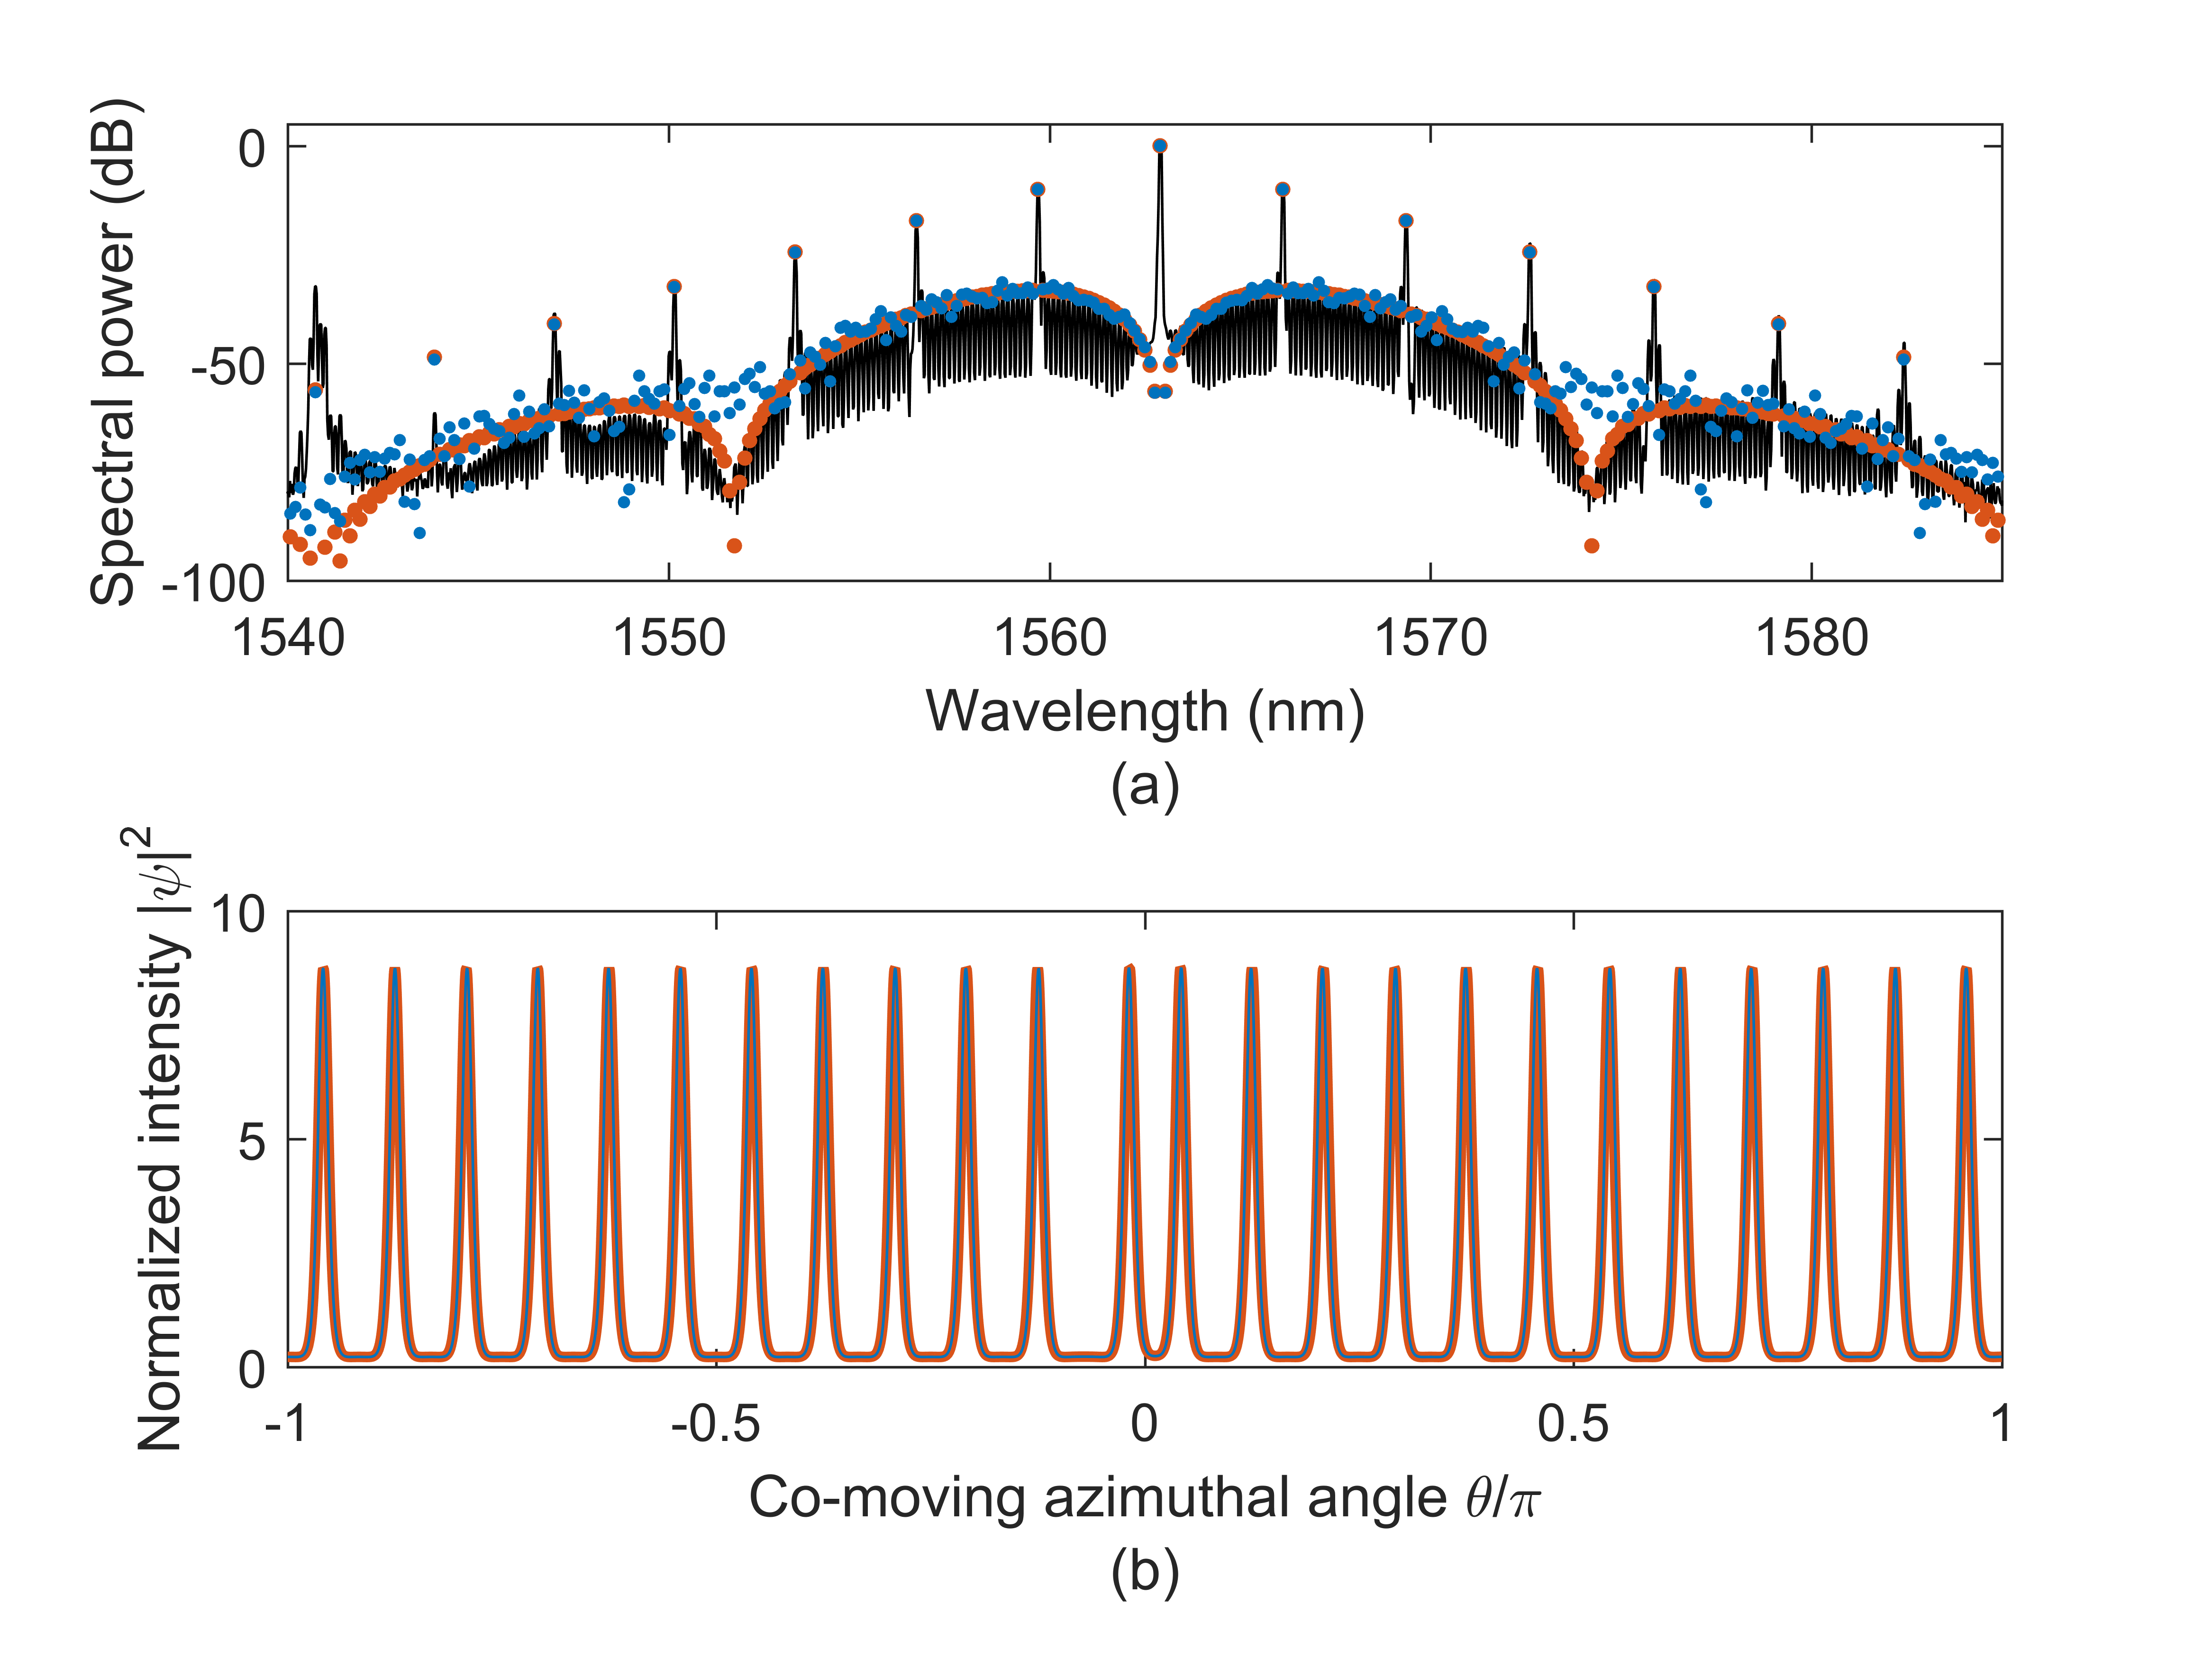
\includegraphics{\FigPath/Figures/SolitonCrystals/SCjiggled_v2.png}
	\end{center}
	\caption[Spectral contrast of a soliton crystal]{\textbf{Spectral contrast of a soliton crystal.} (a) Experimental measurement of a soliton-crystal spectrum (black), along with spectra corresponding to two approximations to the crystal's time-domain waveform as a soliton ensemble, according to Eq. \ref{eq:LLEsolens}. Shown in orange is the spectrum of an ensemble of solitons pinned to sites on a lattice with spacing $2\pi/(7\times24)$; here the majority of the pulses are separated from their neighbors by seven lattice sites, but one pulse is displaced by two lattice sites from its expected position. Shown in blue is a calculation of the spectrum that results when random (uniformly distributed) jitter is imposed on the same pulse positions; the range of the jitter is $\pm$ 3 $\%$ of the typical inter-soliton spacing $2\pi/24$. (b) Time-domain traces corresponding to the spectra shown in (a). There is no readily apparent difference between the positions of the pulses in two pulse trains because the magnitude of the imposed jitter is small; nevertheless the definition of the distinctive spectral features is eroded by the jitter.}
	\label{fig:SCjiggled}
\end{figure} 

We present plots illustrating the spectral and temporal characteristics of an example soliton crystal in Fig. \ref{fig:SCjiggled}. Fig. \ref{fig:SCjiggled}a shows an experimental measurement of a soliton crystal spectrum. This spectrum exhibits prominent comb modes similar to primary-comb lines, and underlying these primary-comb lines are single-FSR-spaced spectral lobes. It is possible to understand how the characteristics of this spectrum arise from a well-ordered ensemble of solitons using the basic properties of the Fourier transform, so here we consider construction of this spectrum in a thought experiment: We begin with the primary comb spectrum with spacing $N\times f_{FSR}$, which corresponds to a train of $N$ uniformly spaced pulses in the resonator; here $N=24$. To this pulse train we add an \textit{out-of-phase} pulse $S_-$ that coincides in time with one of the existing pulses---in the time domain this corresponds to the introduction of a vacancy into the pulse train, while in the frequency domain this corresponds to the addition (in the phase-sensitive field quantity) of the primary-comb spectrum and the spectrum of the single, out-of-phase soliton. We then add a second soliton $S_+$  to the pulse train, this one \textit{in phase} with the existing pulses and slightly temporally shifted from the vacancy. The time-domain result is a pulse train with one pulse displaced from its expected position based on uniform spacing. In the frequency domain, the positions of the pulses $S_+$ and $S_-$ correspond to different linear spectral phase shifts on each of their individual spectra; when these spectra are added together the result is spectral interference that is periodic in frequency. This gives rise to the lobes beneath the primary-comb lines; the frequency period of the interference is inversely proportional to the separation between the pulses $S_+$ and $S_-$ in time.


We illustrate this principle by plotting pulse trains exhibiting a shifted pulse in Fig. \ref{fig:SCjiggled}b, and show their calculated spectra in Fig. \ref{fig:SCjiggled}a. These pulse trains are constructed using the analytical approximation to soliton ensembles provided by Eq. \ref{eq:LLEsolens}. The pulse train shown in orange is composed of solitons pinned to sites on a lattice, and the pulse train shown in blue is obtained from this first pulse train by introducing a small random displacement to the position of each pulse. The effect of this small position jitter is apparent in the calculated spectra in Fig. \ref{fig:SCjiggled}a---the highly-distinctive spectral characteristics of the soliton crystal are eroded. In fact, it is a general property of the soliton-crystal spectra that we present in this chapter that the contrast and definition of the distinctive spectral characteristics depend on the high precision with which the pulses fall on the lattice sites.



\section{Soliton crystal generation}

Soliton crystals are characterized by stable, dense occupation of the resonator by soliton pulses, and this dense occupation comes with high circulating power relative to single solitons or few-soliton ensembles. This important fact allows soliton crystals to be generated with decreasing pump-laser frequency scans across the resonance that are adiabatic---slow enough that both the resonator temperature and the state of the comb $\psi$ are maintained at values\footnote{This terminology is a bit imprecise when applied to chaotic Kerr-combs that evolve with time; in this case the chaos exhibits the behavior at each point in the scan that would be expected if $\alpha$ and $F^2$ were held fixed.} that correspond to the instantaneous $\alpha$ and $F^2$ parameters throughout the scan. We demonstrate generation and experimental characterization of a soliton crystal in Fig. \ref{fig:SCexample}. It is interesting to contrast the continuity of the taper-transmission trace with the staircase-like nature of the same measurement exhibited in the generation of a few-soliton ensemble (see e.g. Ref. \citeNoBrackets{Herr2014} and the discussion in Chap. \ref{chap:microresonators}). Slower scans than the one presented in Fig. \ref{fig:SCexample} are possible, and in fact we have generated soliton crystals by tuning the pump-laser frequency arbitrarily slowly by hand.

\begin{figure}[htpb]
	\begin{center}
		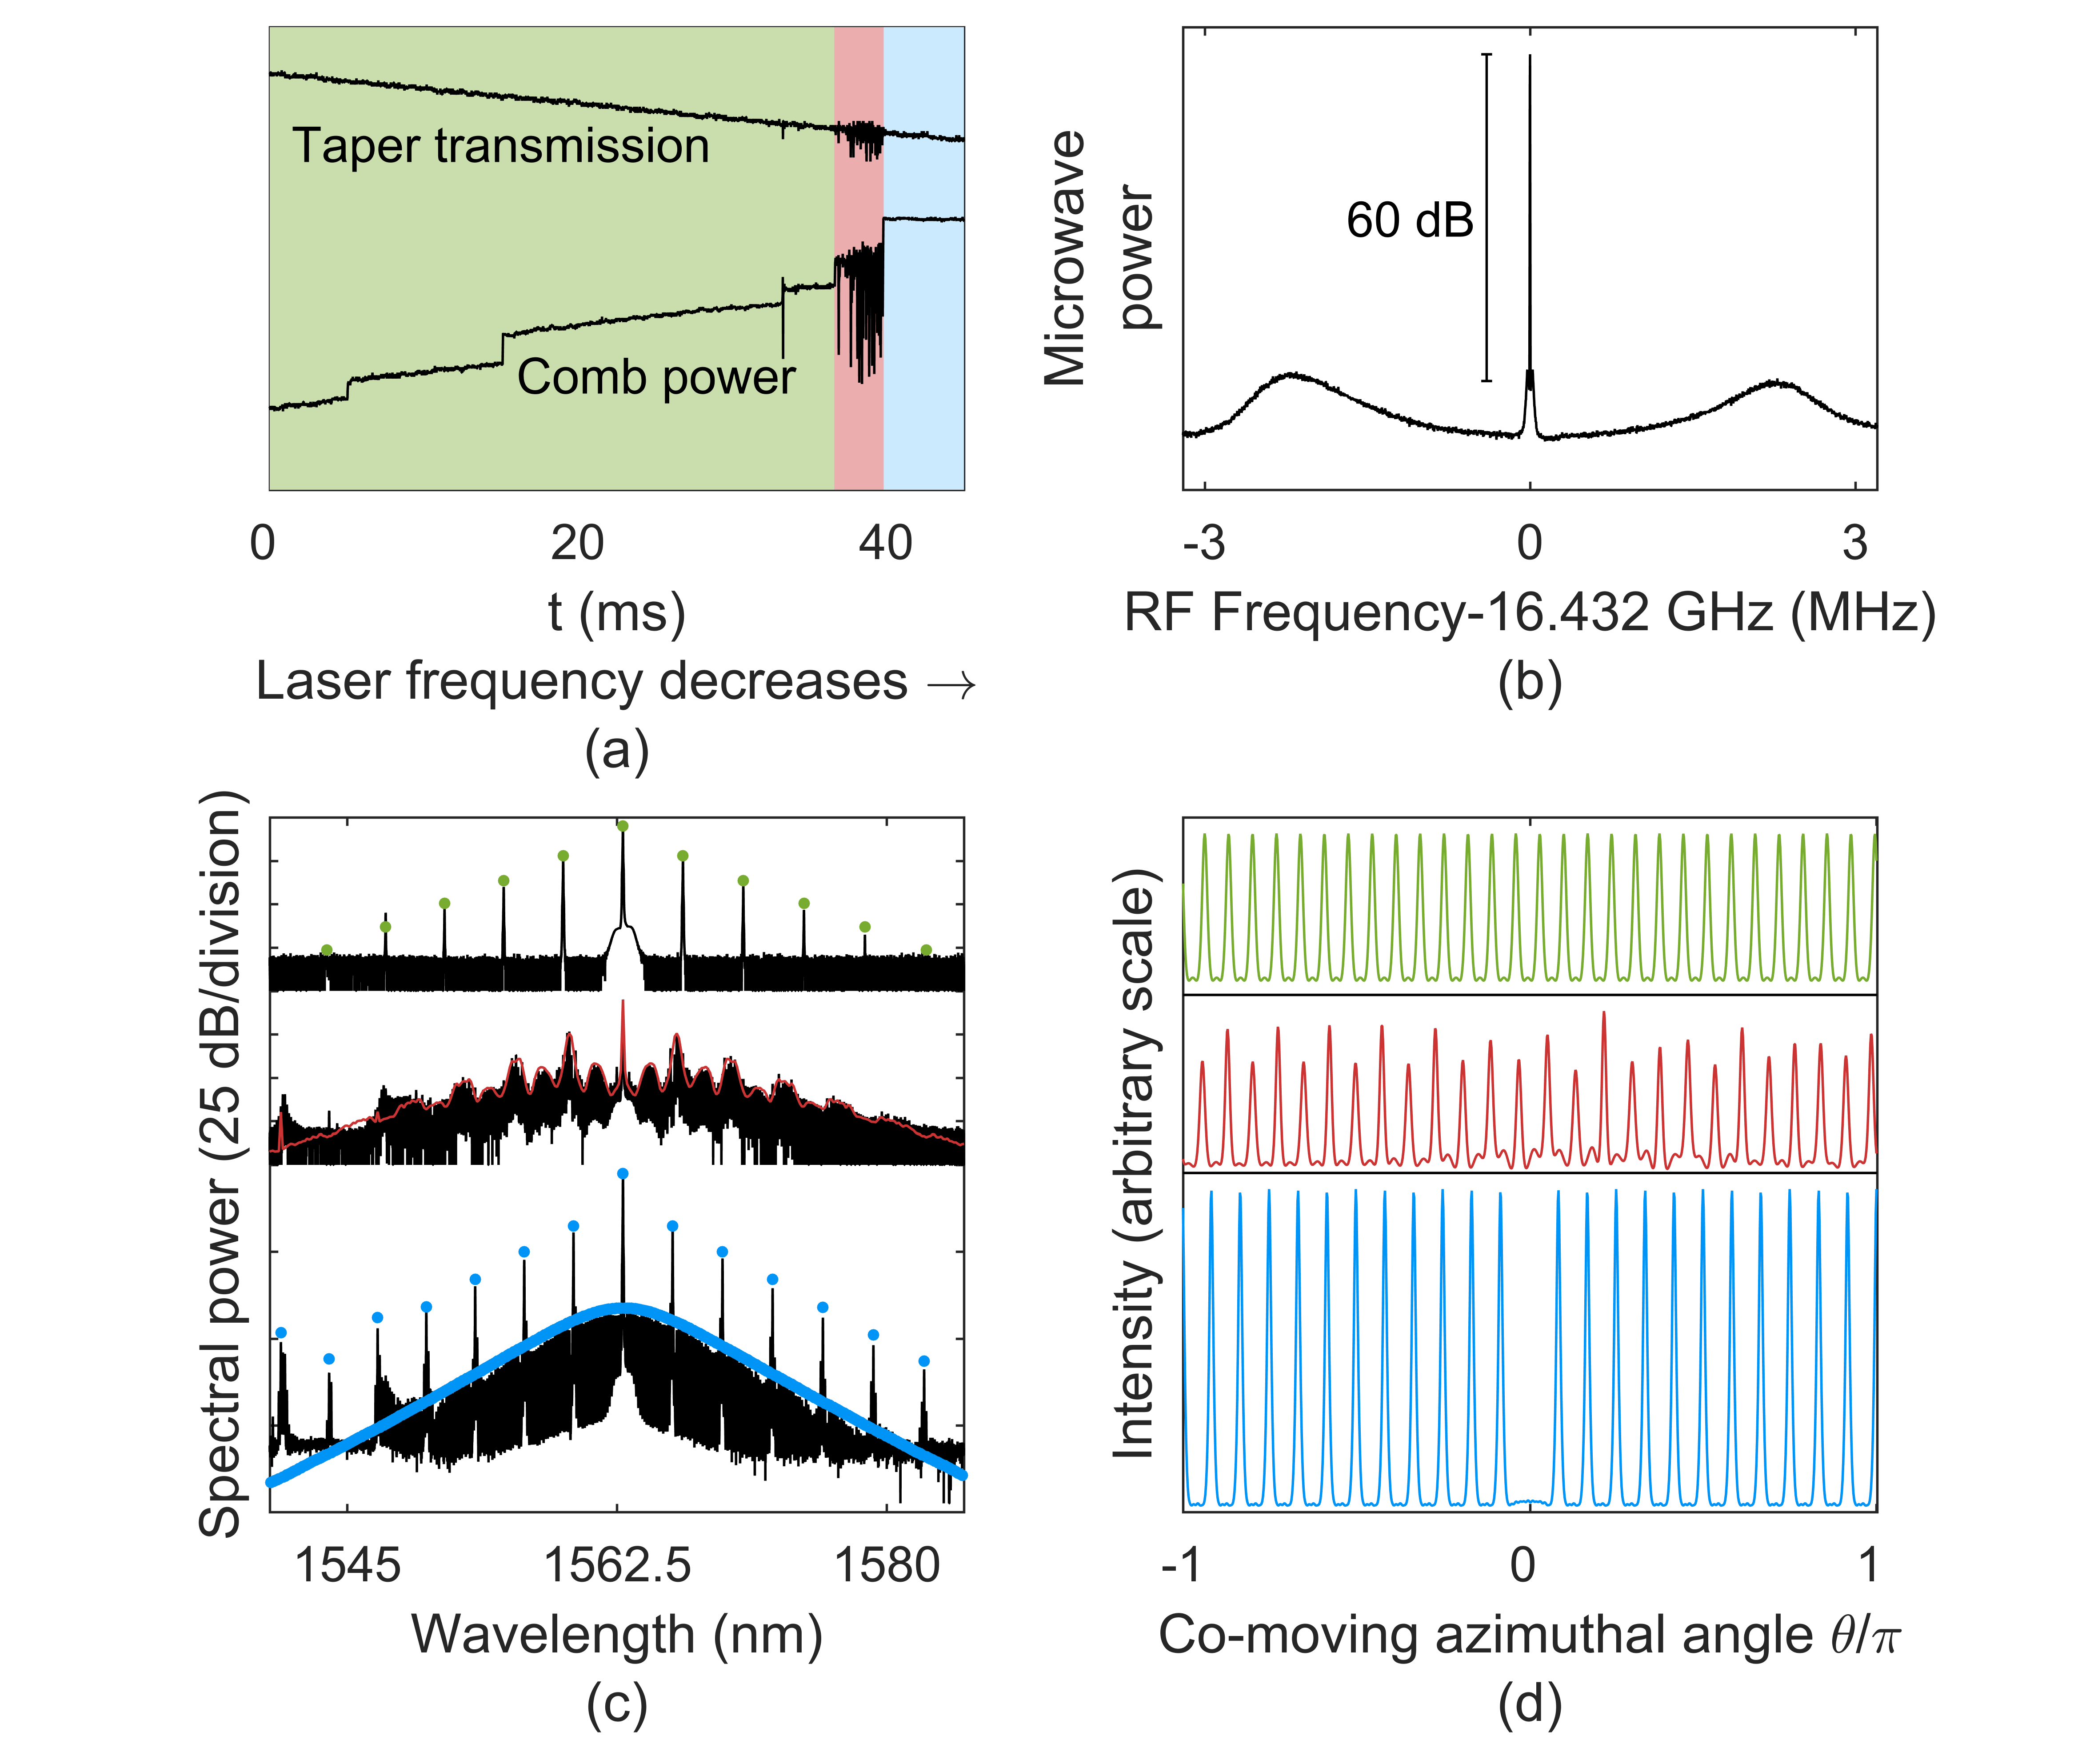
\includegraphics{\FigPath/Figures/SolitonCrystals/SCexample.png}
	\end{center}
	\caption[Generation and characterization of a soliton crystal]{\textbf{Generation and characterization of a soliton crystal.} (a) Measurements of the power transmitted past the resonator (`Taper transmission') and this power with the pump frequency filtered out (`Comb power') during crystal generation with a scan that proceeds through primary-comb (green), chaotic (red), and soliton crystal (blue) regimes. The resonator's thermal response leads to the non-Lorentzian taper transmission profile, and the continuity of the taper transmission trace upon soliton crystal condensation indicates that the intracavity power of the soliton crystal is matched to the chaos that precedes it. (b) Narrow measured RF beat for the repetition rate of the soliton crystal is indicative of a coherent comb, in contrast with the chaotic state. (c) Progression of the optical spectrum through the scan, with experimental data (black) obtained by halting the scan at the appropriate point, and LLE simulations (with a perturbation as described in Sec. \ref{sec:crystallizationmechanism}) in color. The simulated spectrum for the chaotic state shown in red is a time average. (d) Simulated time-domain traces corresponding to the simulated spectra in (c). The simulated intensity for the chaotic state is a snapshot. The soliton crystal shown in blue is a uniform pulse train with a single vacancy (see text).}
	\label{fig:SCexample}
\end{figure} 

\section{Mechanism of soliton crystallization} \label{sec:crystallizationmechanism}

%Figs. \ref{fig:SCexample}c and d present the optical spectrum and simulated corresponding time-domain waveform of a soliton crystal. This spectrum consists of widely-spaced primary-comb lines that are separated by many resonator FSR superposed with an underlying $\mathrm{sech}^2$ spectrum of the kind that corresponds to a single soliton. In fact, this spectrum can be understood through the basic superposition principle of the electric field: The primary comb spectrum with spacing $N\times f_{FSR}$ corresponds to a train of $N$ uniformly spaced pulses in the resonator. The observed crystal spectrum corresponds to such a pulse train with a single vacancy, where a pulse is missing. The effect of this vacancy on the spectrum can be understood by considering the addition of an \textit{out-of-phase} pulse $S_-$ to a primary-comb pulse train, where $S_-$ coincides in time with one of the existing pulses---in the time domain this corresponds to removal of one of the pulses, while in the spectral domain this corresponds to the addition (in the phase-sensitive field quantity) of the primary-comb spectrum and the spectrum of the single, out-of-phase soliton. The soliton crystal spectrum shown in Fig. \ref{fig:SCjiggled} can also be understood this way: If a second soliton $S_+$ is added to the initial primary-comb pulse train, this one \textit{in phase} with the existing pulses and slightly temporally shifted from the vacancy, the result is a pulse train with one pulse displaced from its expected position based on uniform spacing. In the frequency domain, the positions of the pulses $S_+$ and $S_-$ correspond to different linear spectral phase shifts on each of their individual spectra; when these spectra are added together (in the phase-sensitive field quantity) the result is spectral interference that is periodic in frequency. This gives rise to the lobes beneath the primary-comb lines; the period (in frequency) of the interference is inversely proportional to the separation between the pulses $S_+$ and $S_-$ in time.

The time-domain waveforms we have considered so far are not stable in evolution under the LLE. For each, the observed width of the spectrum fixes the ratio between $\alpha$ and $\beta_2$, as seen from Eq. \ref{eq:LLEsoliton}. This ratio then fixes the temporal duration of the solitons, in turn determining the characteristic length of their interactions. When an attempt to simulate the crystal according to the LLE is made with parameters that give agreement with the measured width of the optical spectrum (e.g. $F^2$=3.7, $\alpha=3.77$, and $\beta_2=-0.0054$ for the crystal in Fig. \ref{fig:SCexample}c and d), it is found that pair-wise attractive interactions between solitons lead to collapse of the crystal, as shown in Fig. \ref{fig:SCexamplesim}.

A stabilization mechanism that goes beyond the physics of the LLE is responsible for the stability of soliton crystals. The stabilization mechanism for the crystals we present here arises from avoided mode crossings in the resonator spectrum. As discussed in Sec. \ref{sec:OMRR}, the resonators used in these experiments support multiple families of circulating modes, each with its own transverse spatial intensity profile and free spectral range. Although the modes in different families are in principle orthogonal, coupling between them can be provided by perturbations, for example by the coupling waveguide or tapered fiber used to drive the resonator, or anomalies in the resonator fabrication that break the resonator symmetry. When a coupling exists between modes that are sufficiently close in frequency, the modes become hybridized and their frequencies become displaced \cite{Haus1991}. The effect of this coupling and the associated perturbation to the resonator mode spectrum on Kerr-comb generation has been investigated \cite{Savchenkov2012}, and it has been found that avoided mode crossings can inhibit soliton generation in anomalous-dispersion resonators \cite{Herr2014a,Yi2015}, while they can facilitate the formation of Kerr-combs in normal-dispersion resonators \cite{Liu2014a,Xue2015,Bao2017}. 


%A `mode family' corresponds to a set of circulating modes that have different azimuthal mode numbers but (approximately, neglecting wavelength-dependent effects) the same transverse spatial mode profile. As discussed in Sec. \ref{sec:ec;OMRR}, some resonators support multiple mode families, each with its own free spectral range at a given wavelength. If a coupling exists between two modes that are sufficiently close in frequency, the frequencies of the modes become displaced from their frequencies in the absence of this coupling \cite{Haus1991}. This affects Kerr-comb generation in the affected mode families, because the local detuning between the resonator modes and the Kerr-comb modes is changed as a result of the mode crossing. This comb-resonator detuning change may either enhance or inhibit nonlinear frequency conversion to the effected Kerr-comb modes, thereby changing the amplitude of these modes in the comb spectrum. 

Here we are interested specifically in the impact of an avoided mode crossing on the temporal waveform of a soliton. For simplicity, we make the approximation that a single mode of the Kerr comb with number $\mu_\times$ is affected by the mode crossing; as we will see, this number $\mu_\times$ determines the spacing between the lattice sites $\theta_n$ defined in Sec. \ref{sec:crystalbasics}. The approximation of perturbation of a single mode by the mode crossing neglects the fact that avoided mode crossings between two families typically span a range of modes. This occurs because mode families that have a small fractional difference in free-spectral range between them traverse each other slowly in the frequency domain; this can be observed in many of the experimental spectra presented in this chapter. However, we find that the single-mode assumption is generally sufficient for modeling the stability of the soliton crystals that we observe.

The perturbation of the frequency of a resonator mode $\mu_\times$ that is far from the pumped mode $\mu=0$ affects the local detuning of the comb from the resonator. When this local comb-resonator detuning is decreased, the efficiency of nonlinear frequency conversion to mode $\mu_\times$ can be increased. This increases the amplitude of mode $\mu_\times$ in the soliton's spectrum, and the resulting change to the time-domain waveform can be understood by considering this increase as the addition of extra CW light at the frequency of mode $\mu_\times$. This extra CW light leads to the introduction of periodic intensity oscillations in the background on which the soliton rides as it beats against the existing background at the pump frequency. The new background wave in the cavity has a period of $2\pi/\mu_\times$ in the angular coordinate $\theta$.

When several of these perturbed solitons co-propagate in a resonator, they interact through their extended waves and arrange themselves such that the waves constructively interfere \cite{Wang2017}. Each soliton then lies at the peak of a single extended background wave in the resonator, similar to predictions for bichromatically pumped Kerr combs \cite{Hansson2014}. Importantly, temporal separations between solitons are therefore required to be multiples of this wave's period; equivalently, solitons must lie on lattice sites with relative positions (i.e. up to an overall shift of the crystal) defined by $\theta_n=2\pi n/\mu_\times$. The background wave stabilizes the crystal against attractive interactions. Furthermore, the wave's amplitude, and thus the strength of the crystal against perturbations, increases with the number of co-propagating perturbed solitons. Within the assumption of single-mode perturbation of the comb's spectrum, this interaction has infinite range. 

We note that the mechanism observed here builds on previous reports of related phenomena. It has been shown that local interactions between cavity solitons can arise through decaying oscillatory tails \cite{Skryabin1999}, leading to the formation of small, locally ordered soliton molecules; this effect appears to be significant in Kerr ring resonators only at small detunings \cite{Parra-Rivas2017}. Additionally, it has been shown that the injection of a second CW laser into a passive fiber-ring resonator can result in the generation of uniform distributions of solitons \cite{Wabnitz1996}. The mechanism we report here can be viewed as a variant of this CW-soliton interaction in which the `injected' CW laser is provided by the solitons themselves through the affect of the mode crossing on the solitons' spectra.

We connect this discussion to the soliton-crystal spectrum presented in the bottom trace of Fig. \ref{fig:SCexample}c---this spectrum exhibits excess power near modes $\mu_{\times,1}=5\times24=120$ (1547 nm) and $\mu_{\times,2}=7\times24=168$  (1541 nm), where 24 FSR is the spacing of the prominent primary-comb lines. Also visible is suppressed comb generation where the comb-resonator detuning has been increased. 

\subsection{Simulation of soliton crystals}

To incorporate the stabilization mechanism described above into numerical simulations, we insert into the LLE a reduced comb-resonator detuning on a single mode $\mu_\times$. The mode-dependent comb-resonator detuning can be calculated as:
\begin{align}
\alpha_\mu&=-2(\omega_p+\omega_\mu-D_1)/\Delta\omega,\\
&=\alpha-\beta_2\mu^2/2.
\end{align}

Here $\omega_p$ is the frequency of the pump laser, $\omega_\mu$ is the set of cavity resonance frequencies referenced to the pumped mode, and $D_1=\partial\omega_\mu/\partial\mu|_{\mu=0}$ is the resonator's FSR at the pumped mode and is also assumed to be the comb's repetition rate. The dispersion operator is applied in the frequency domain in numerical simulations of the LLE (see Appendix \ref{app:numericalsims}), which facilitates inclusion of $\delta$-function perturbations to the comb-resonator detuning as:
\begin{equation}
\alpha_\mu=\alpha-\beta_2\mu^2/2+\Delta\alpha_\mu,
\end{equation}
where
\begin{equation}
\Delta\alpha_\mu=2(\omega_\mu-\omega_{\mu,0})/\Delta\omega
\end{equation}
is the normalized change in the frequency of mode $\mu$ from the expected frequency $\omega_{\mu,0}$. 

We demonstrate the stabilization mechanism and the simulation method by presenting a simulation of the crystal in Fig. \ref{fig:SCexample}c. The simulation is shown in Fig. \ref{fig:SCexamplesim}. This figure illustrates both the rapid timescale over which the stabilization mechanism acts and the instability of the crystal in the absence of the stabilization mechanism. To explain the stability of this 23-soliton crystal and the apparently exact circumferential spacing of the pulses by $2\pi/24$ radians, it is sufficient to incorporate into the LLE a reduced comb-resonator detuning on only mode 120 or on mode 168, where the excess power is largest. The crystal is then a steady-state solution of the resulting perturbed LLE.

%We note that a phenomenological application of coupled-mode theory \cite{Haus1991} could be used to calculate the full perturbation to the soliton spectrum by the mode crossing, 

\begin{figure}[htpb]
	\begin{center}
		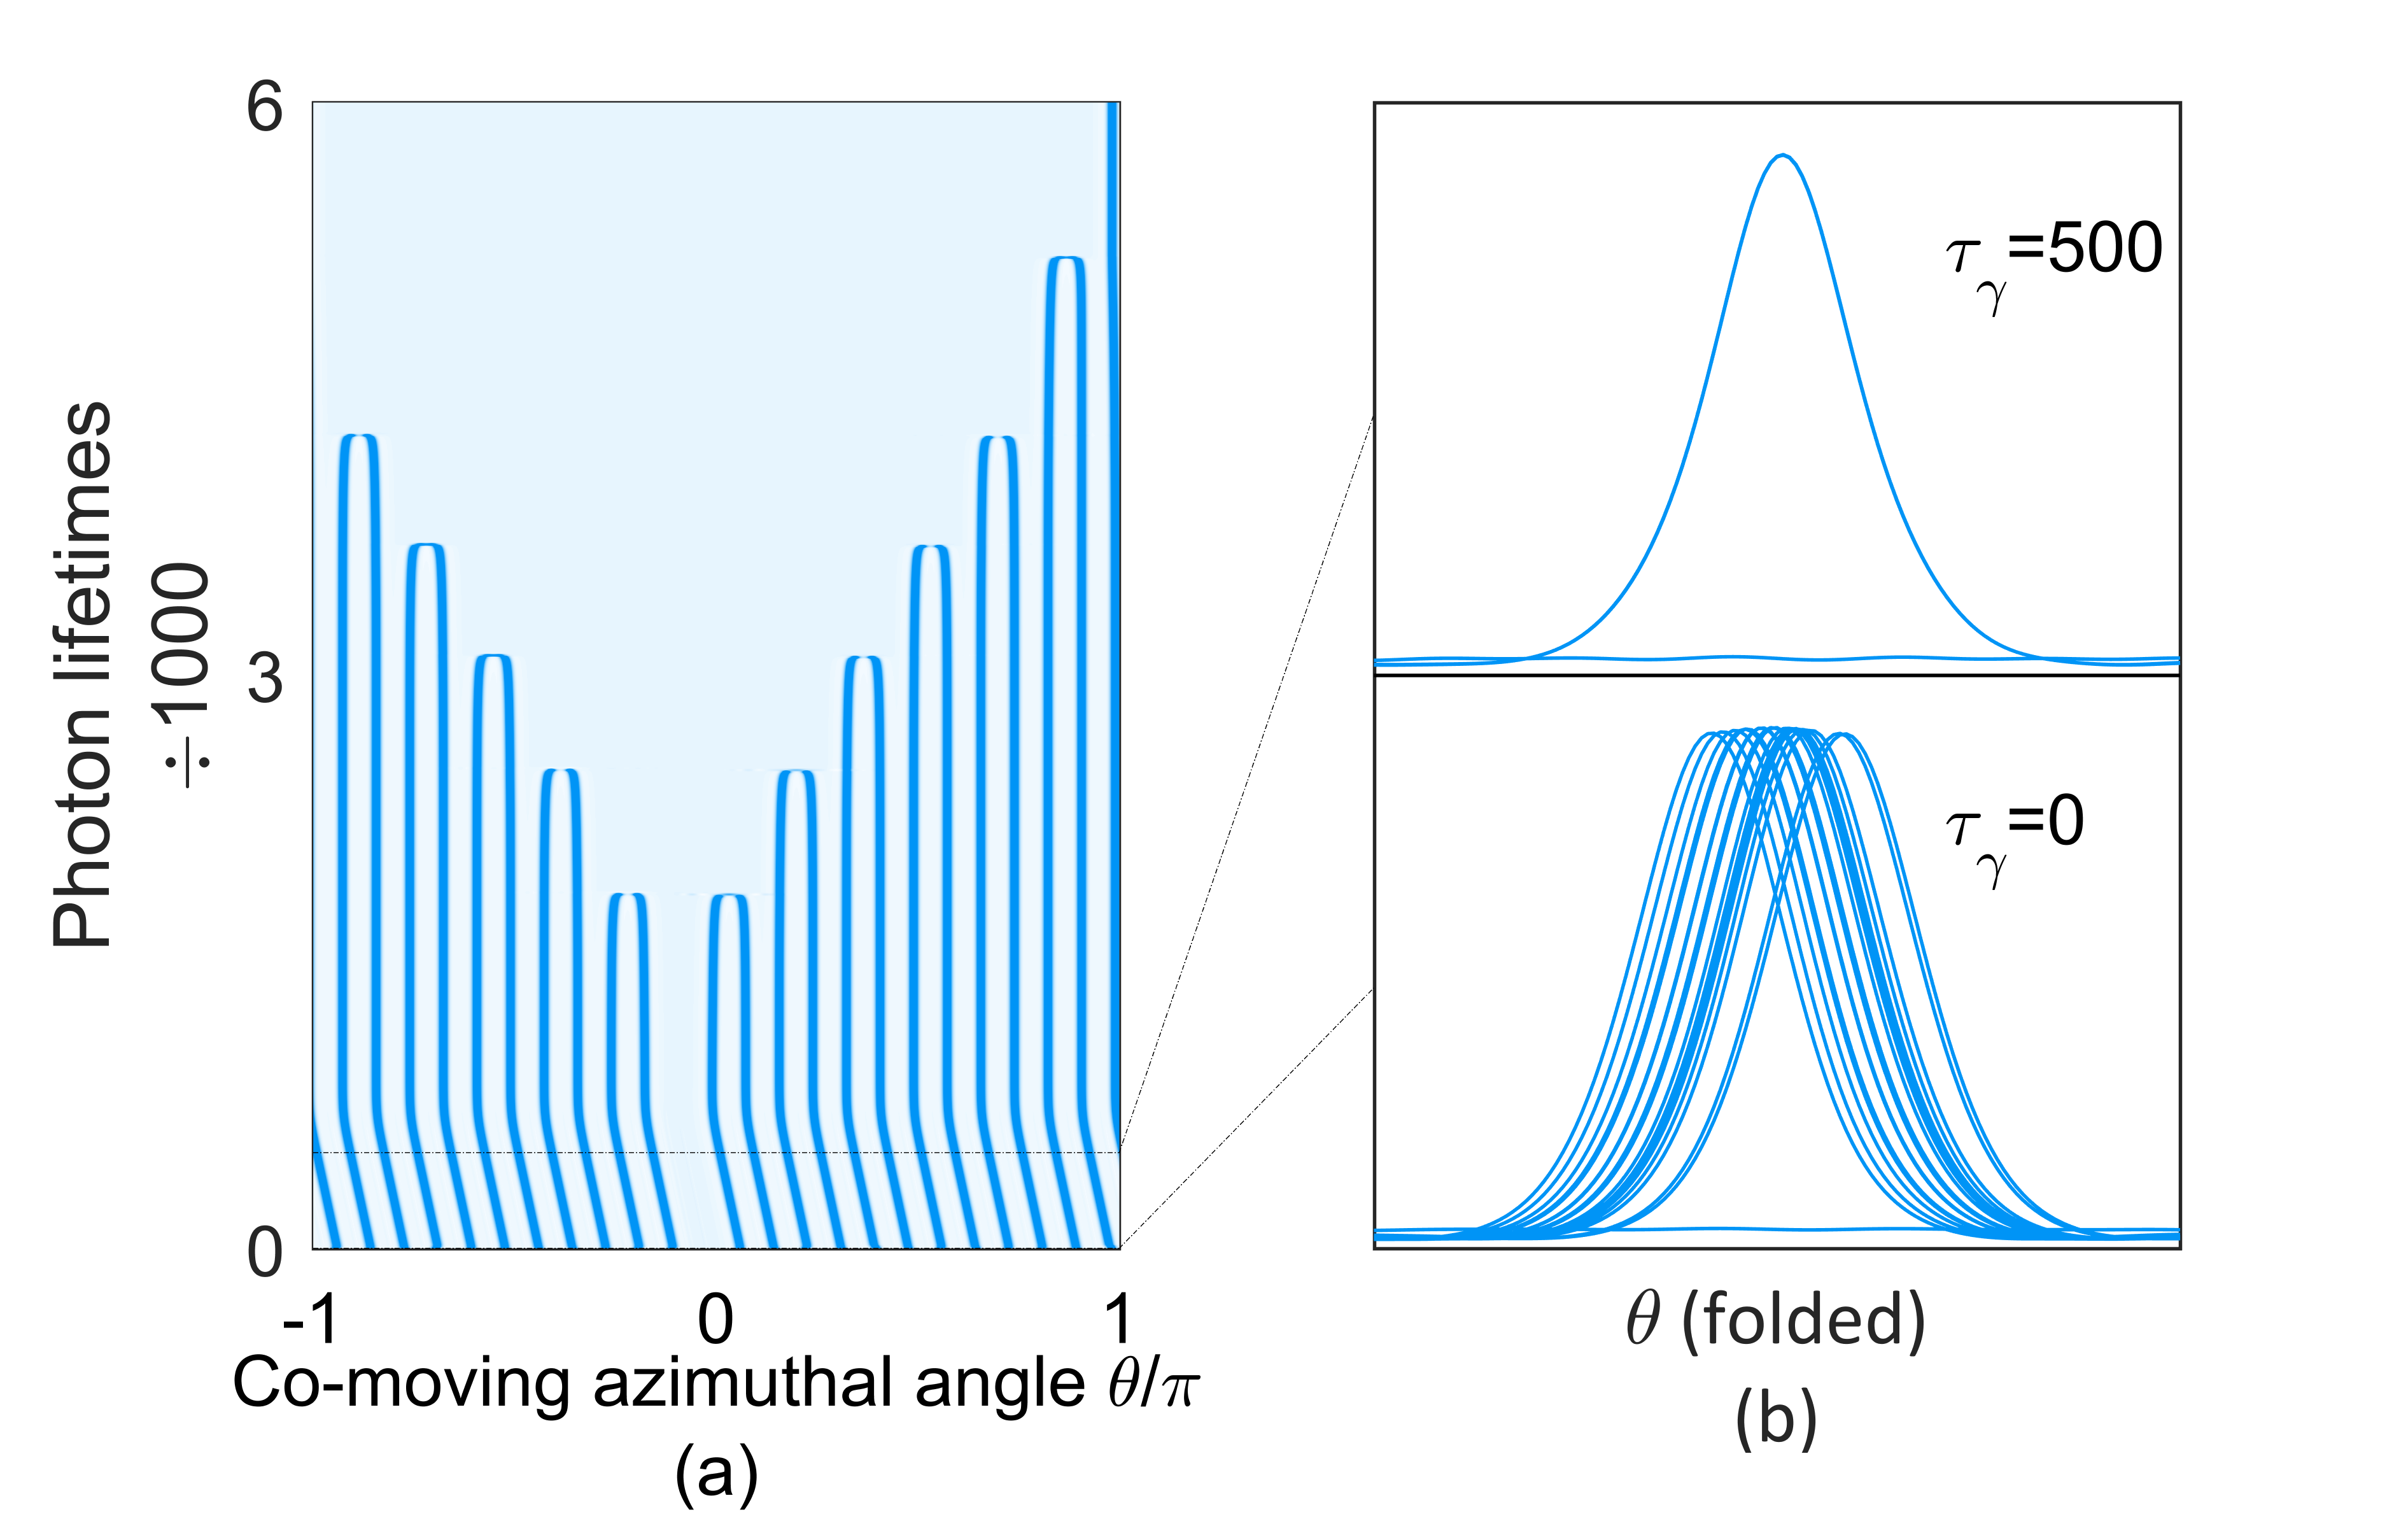
\includegraphics{\FigPath/Figures/SolitonCrystals/SCexamplesim.png}
	\end{center}
	\caption[Stabilization and collapse of a soliton crystal]{\textbf{Stabilization and collapse of a soliton crystal.} (a) Simulated evolution of the pulse train corresponding to the experimental crystal spectrum shown in Fig. \ref{fig:SCexample}c, starting from irregular pulse positions. For the first 500 photon lifetimes of the simulation, the propagation is governed by a perturbed LLE including reduced comb-resonator detuning on modes $\mu_{\times,1}=120$ and $\mu_{\times,2}=168$. The soliton ensemble crystallizes within 10 $\tau_{ph}$ of initialization of the simulation, and then drifts within the co-rotating frame because the additional CW light on modes $\mu_{\times,1}$ and $\mu_{\times,2}$ corresponds to traveling waves. The reduced comb-resonator detuning is removed smoothly from 500 to 1000 photon lifetimes, resulting in the destabilization of the crystal and pair-wise annihilation of the solitons. (b) Intracavity power with the azimuthal coordinate folded modulo $2\pi/24$, demonstrating the initial irregularity of the pulse positions and the crystallized pulse train after 500 photon lifetimes.}
	\label{fig:SCexamplesim}
\end{figure} 


\section{Case study: pair distribution function for a superstructured crystal}

We consider a third specific example of a soliton crystal. The measured and simulated optical spectra for this crystal are shown in Fig. \ref{fig:SCsuperstructure}a. This crystal exhibits superstructure---the soliton pulse train is nearly periodic in a small unit cell but is modulated with a larger periodicity. This results from the frustrated uniform distribution of 16 solitons with allowed inter-soliton separations of $2\pi n/49$ radians; one pair is spaced by $4 \times 2\pi/49$ instead of $3 \times 2\pi/49$ radians.  Excess power is apparent in the spectrum at mode $\mu_\times=49$ (highlighted by the red circle in the plot), and we simulate this crystal phenomenologically by reducing the comb-resonator detuning on mode 49 so that the observed and simulated amplitudes of this mode agree. The total background wave that emerges as the sum of the waves from each constitutent soliton is visible in the plots of the simulated intensity in Fig. \ref{fig:SCsuperstructure}b and c.

\begin{figure}[htpb]
	\begin{center}
		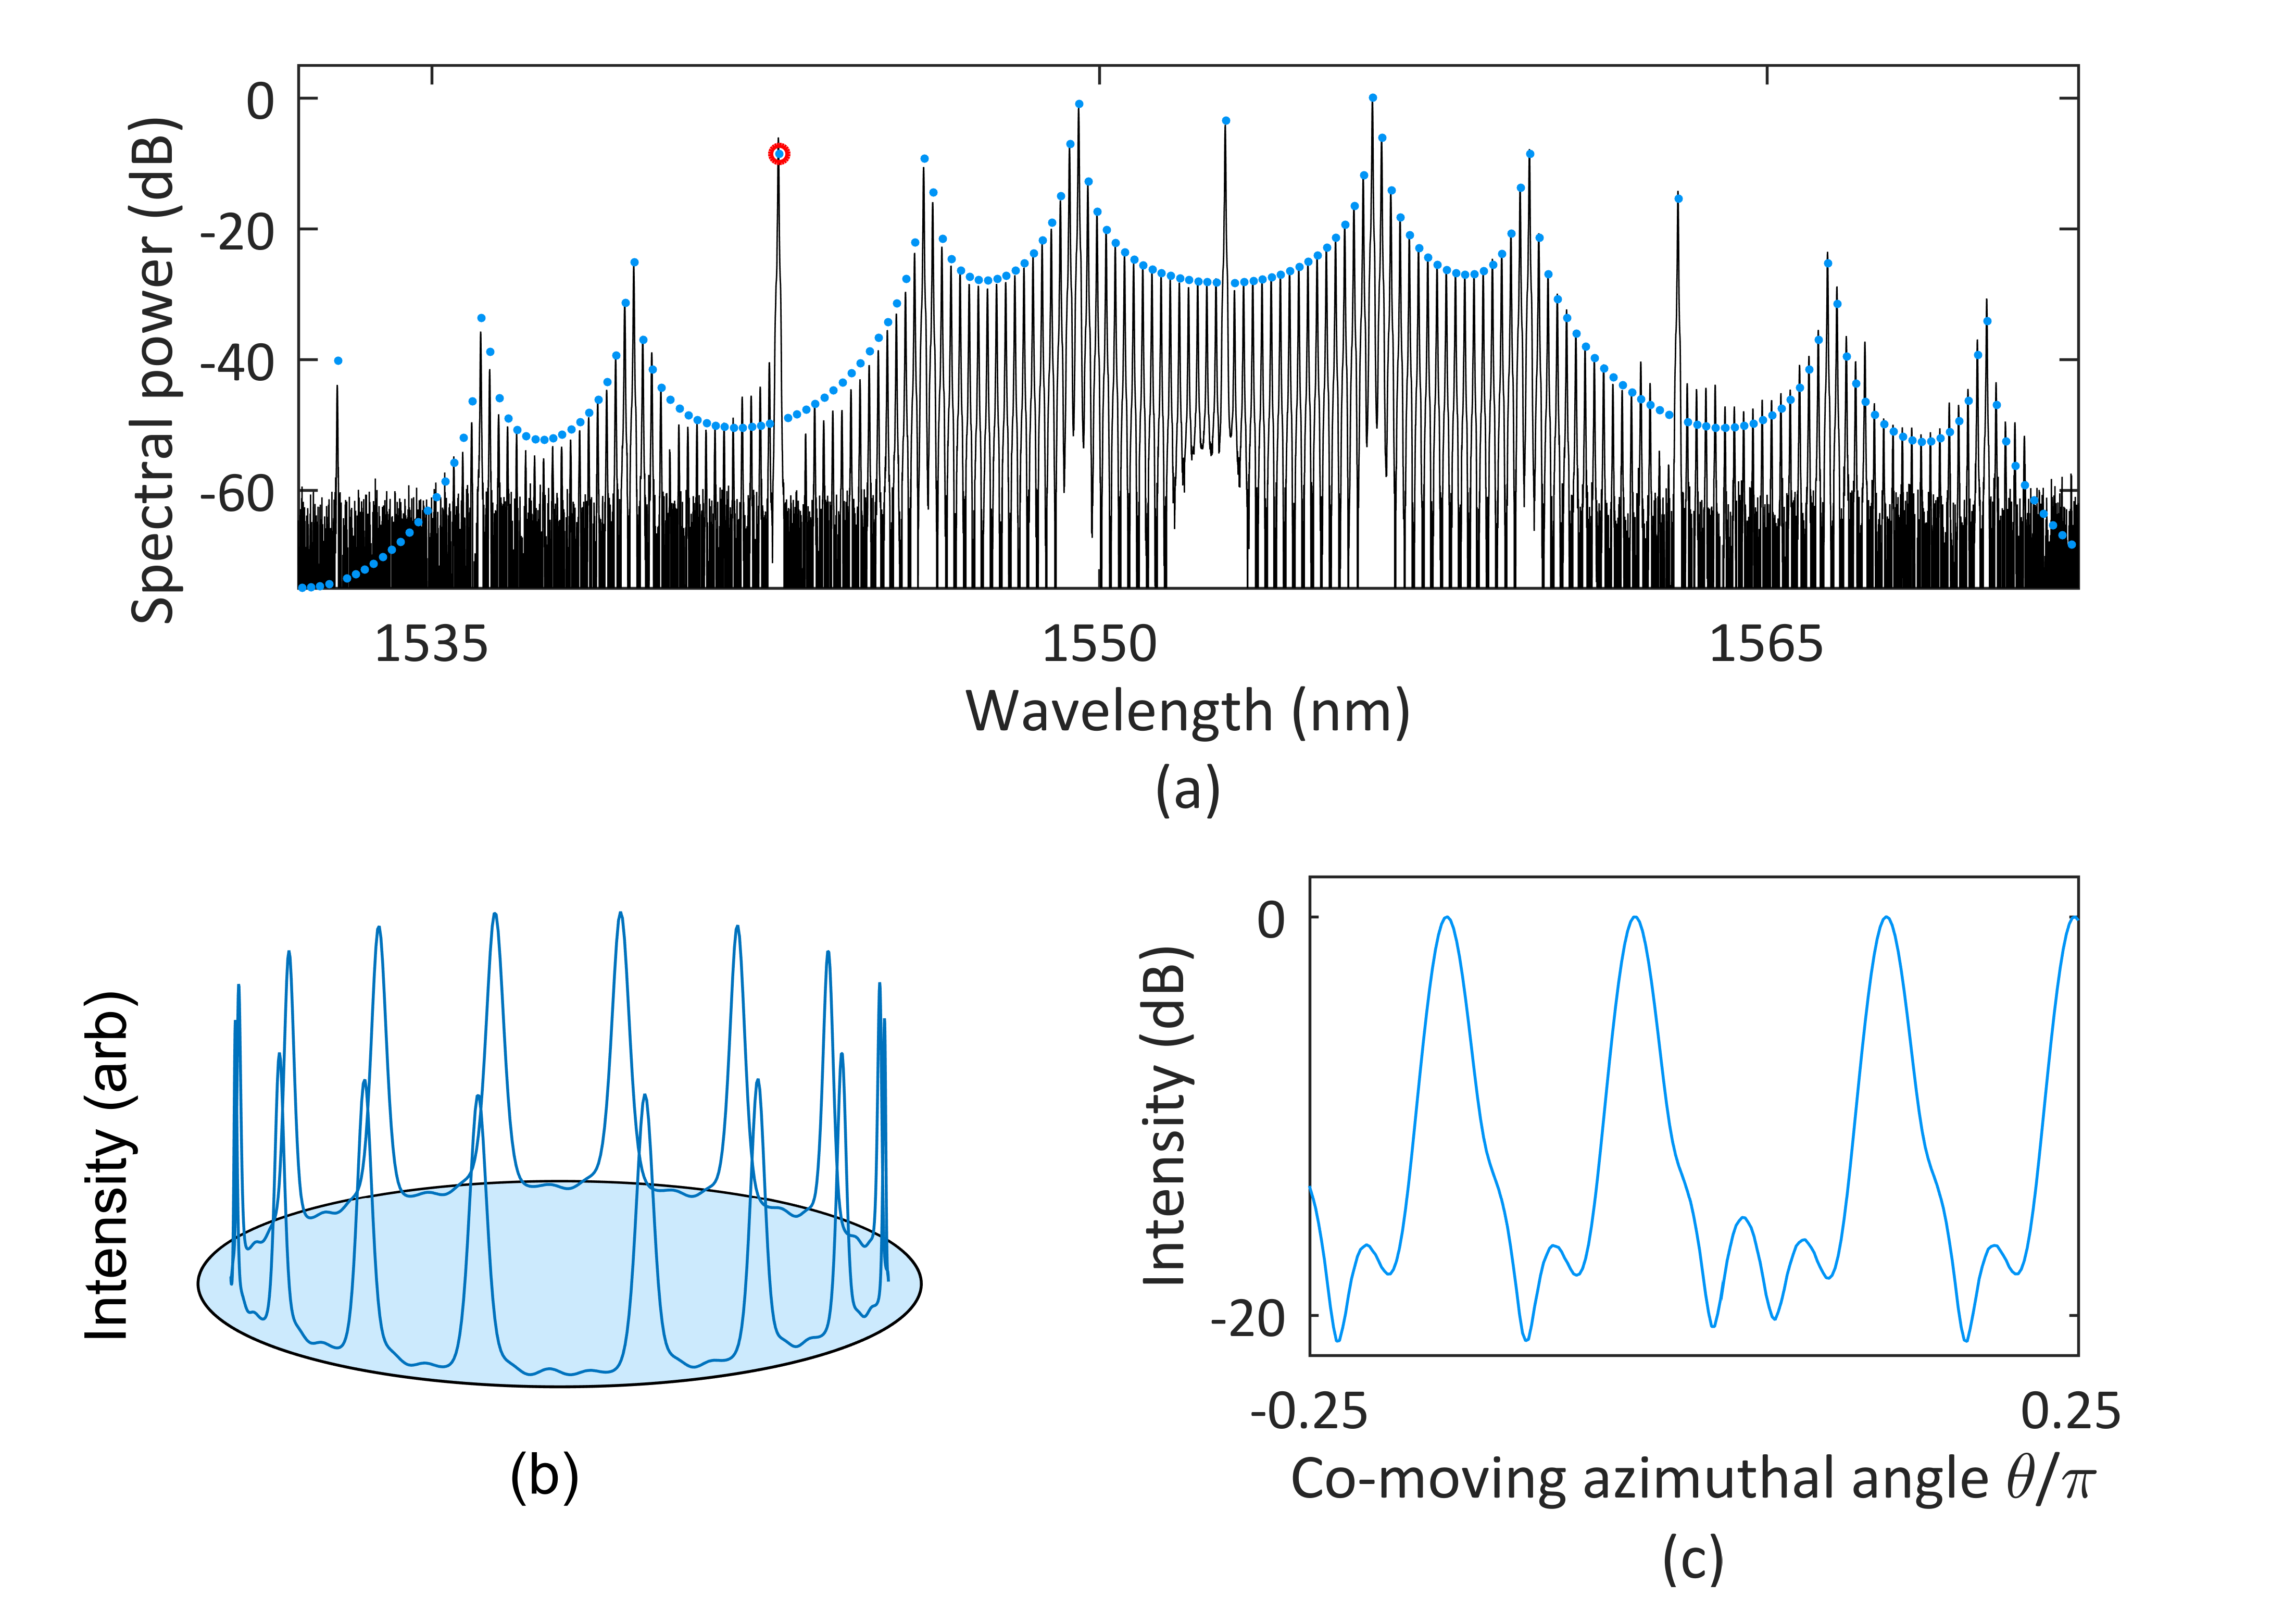
\includegraphics{\FigPath/Figures/SolitonCrystals/SCsuperstructure.png}
	\end{center}
	\caption[Spectrum and waveform of a superstructed soliton crystal]{\textbf{Spectrum and waveform of a superstructured soliton crystal.} (a) Experimental (black) and simulated (blue) optical spectra of a superstructured crystal, with the red dot indicating the mode affected by a mode crossing as described in the text. (b) Simulated time-domain intensity of frustrated-uniform distribution of 16 solitons over 49 lattice points. (c) Zoomed-in logarithm-scale plot of the same that clearly shows unoccupied lattice sites and the anomalous $4\times2\pi/49$ spacing between a pair of pulses.}
	\label{fig:SCsuperstructure}
\end{figure} 

To gain insight into crystal generation, we simulate laser frequency scans across the resonance that generate this crystal in the presence of the mode crossing on mode 49. Example scans are shown for the case without the mode crossing (green) and with it (blue) in Fig. \ref{fig:SCsimgen}. In both scans, solitons emerge from chaos as the frequency of the laser is decreased. In the presence of the mode crossing, they are generated with inter-soliton separations of $2\pi n/49$ radians. A greater number of solitons emerge from chaos in the presence of the mode crossing, and this is consistent with the observed thermal stability of crystal generation in the experiment. Upon continuation of the simulation, some of the solitons in the scan without the mode crossing interact attractively and pair-annihilate, while the crystallized ensemble resulting from the scan with the mode crossing remains stable indefinitely.

\begin{figure}[htpb]
	\begin{center}
		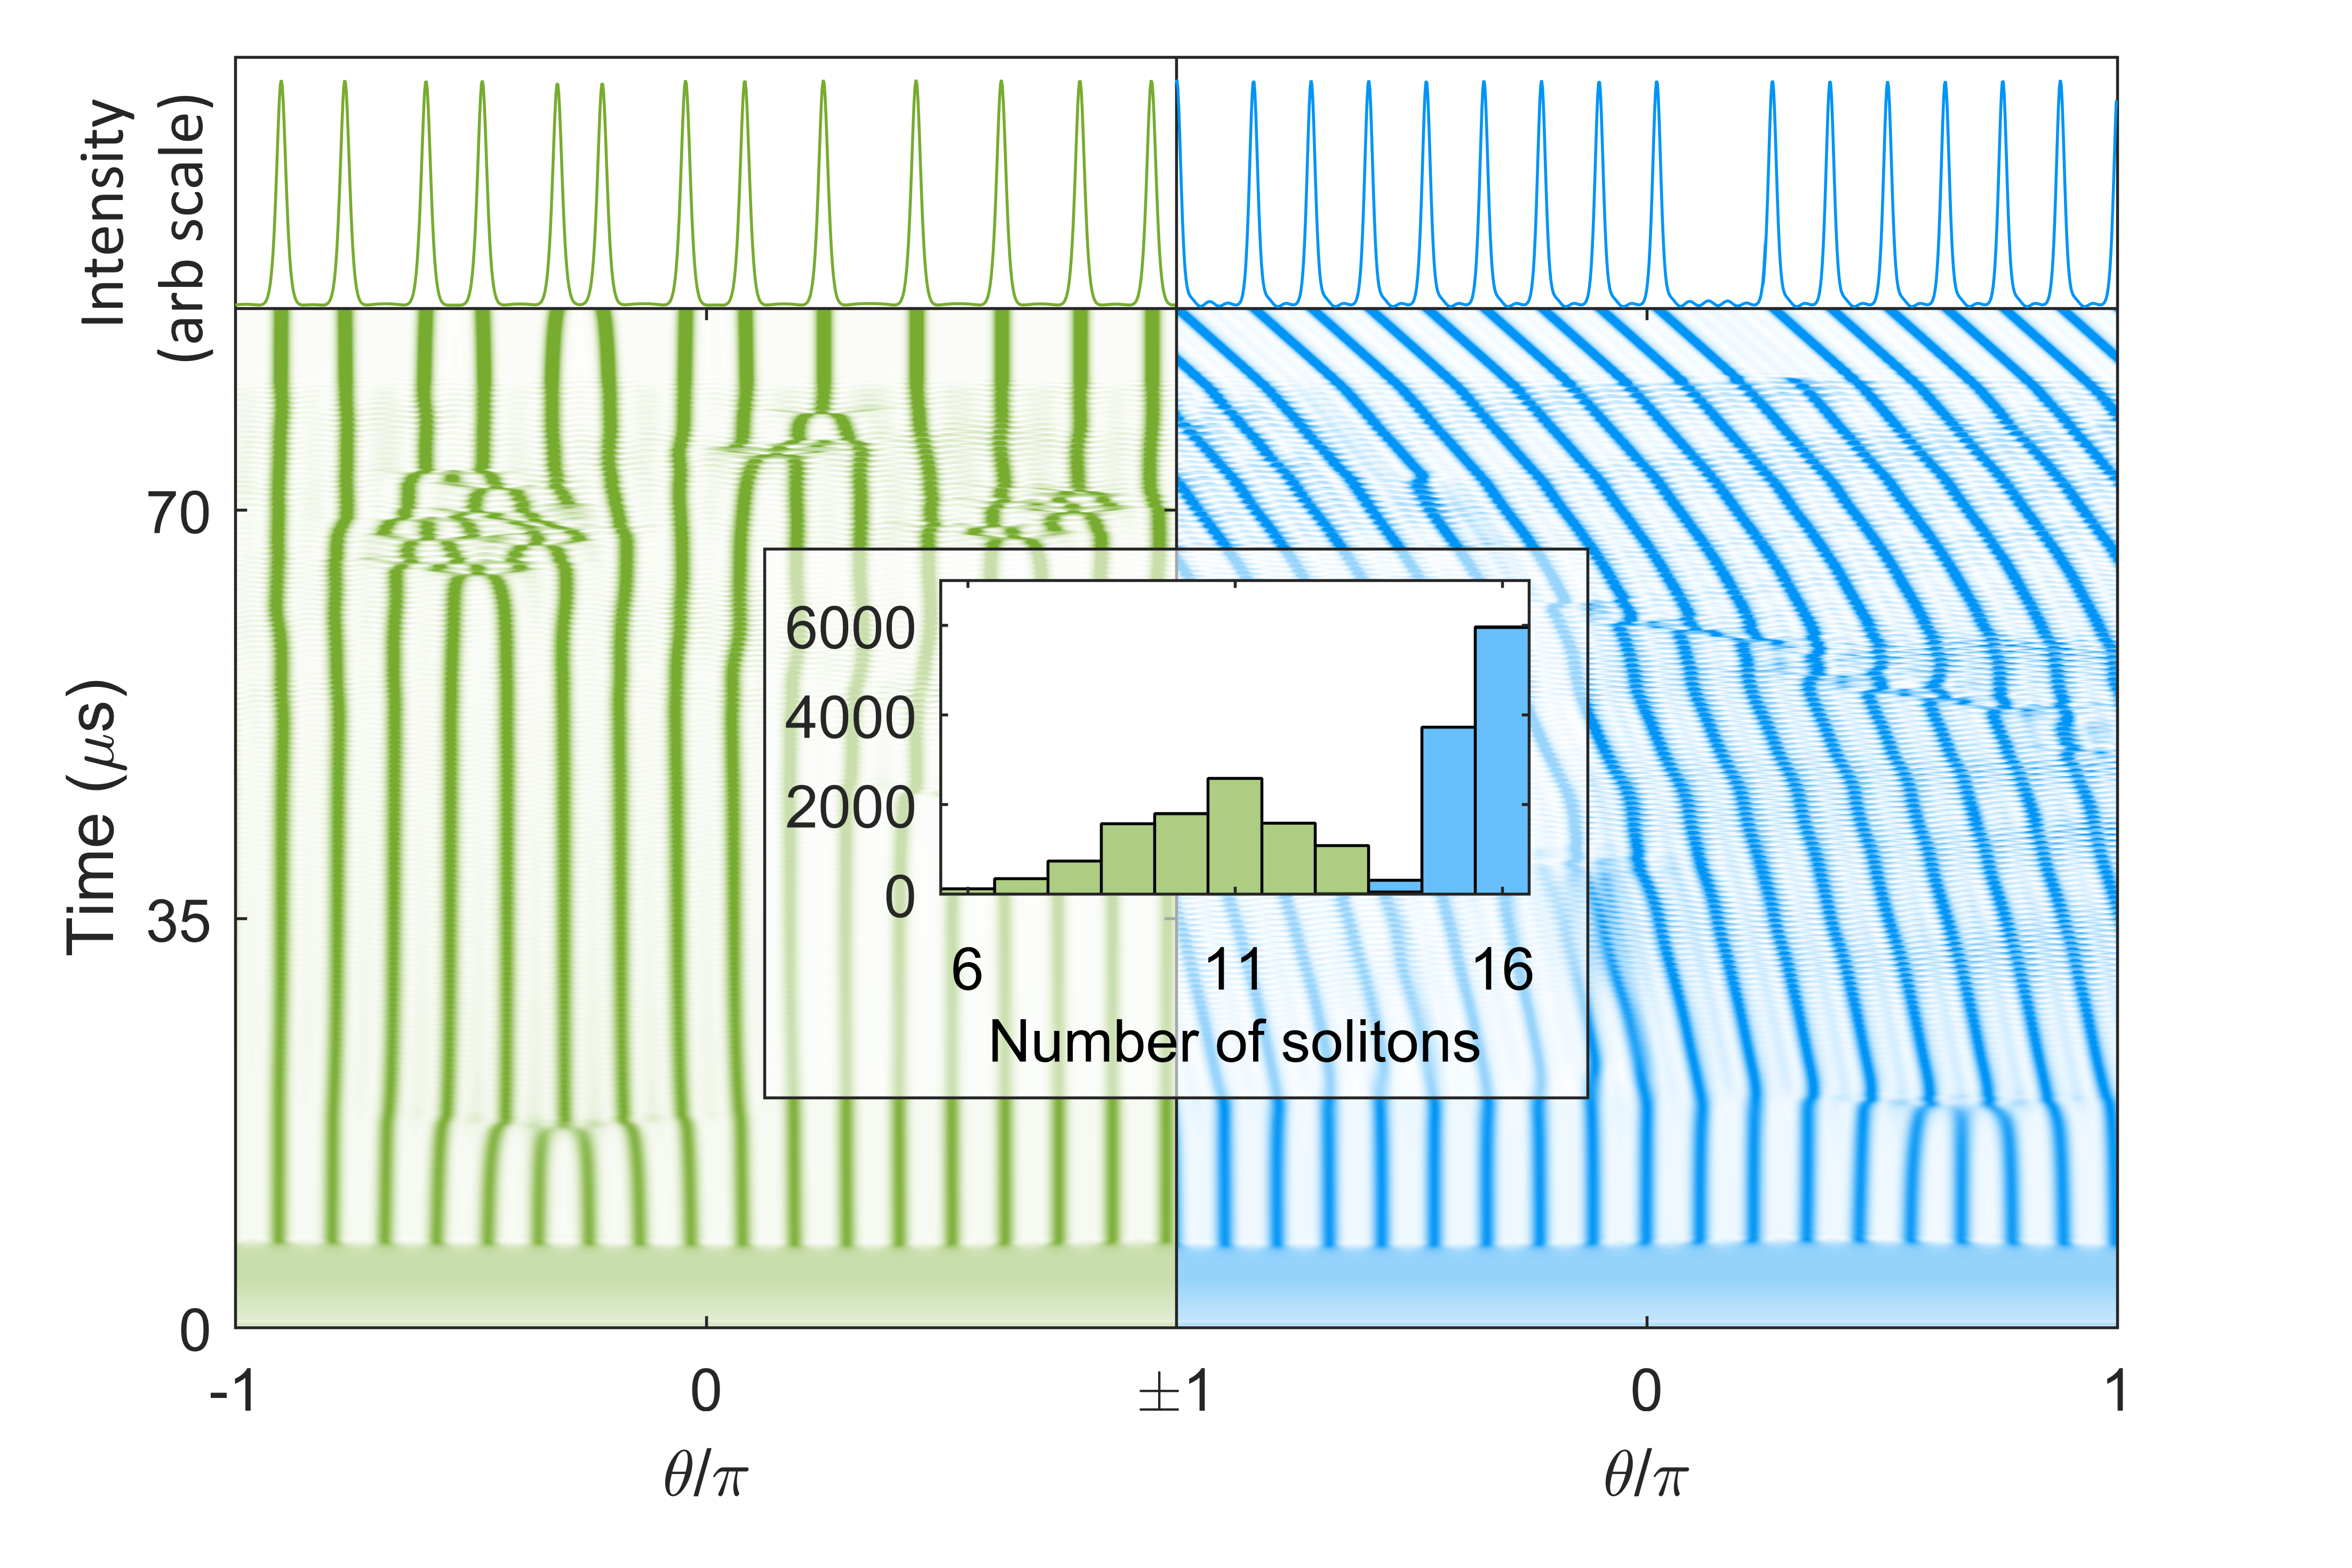
\includegraphics{\FigPath/Figures/SolitonCrystals/SCsimgen.png}
	\end{center}
	\caption[Simulated generation of a superstructured soliton crystal]{\textbf{Simulated generation of a superstructured soliton crystal.} Bottom: plots of the intracavity power during a simulated scan across the resonance, without (green) and with (blue) a mode crossing on mode 49 that reduces the comb-resonator detuning and increases the efficiency of frequency conversion on that mode. Top: final waveforms. Inset: histogram of the number of solitons generated in 10,000 simulated scans.}
	\label{fig:SCsimgen}
\end{figure} 

We investigate the pair distribution function (PDF) for the soliton ensembles generated by these scans. The PDF is the probability that a soliton exists at position $\theta_0+\Delta\theta$ given that a different soliton exists at position $\theta_0$, normalized to the density. This is a useful metric to classify particle interactions that we borrow from condensed matter physics (see e.g. Ref. \citeNoBrackets{Barker1976}, especially Fig. 2, and Ref. \citeNoBrackets{Egami2012}, especially Fig. 1.1 and Chapter 3). We note that for numerically calculated discrete PDFs the absolute scaling of the PDF is not important, as it depends on the density of numerical sampling. In Fig. \ref{fig:SCpdf}, we plot the average PDFs for 10,000 simulated scans with and without the mode crossing. The result for the case with a mode crossing is sharply peaked, indicating that the allowed inter-soliton separations take on discrete values. The result for the case without the mode crossing is continuous, with a peak near the most likely nearest-neighbour separation and periodic revivals at its multiples, falling to the value of the PDF for uncorrelated soliton positions (the density) at large separations. This is exactly the expected form of the PDF for a liquid \cite{Barker1976,Egami2012}. For comparison, we plot a PDF (black) generated by simulation of a simple particle ensemble with mean inter-particle separation of $\Delta\theta=0.155\pi$ and normally distributed noise on this value with standard deviation of $\sigma_{\delta\theta}=0.18\Delta\theta$. Thus, with a particle labeled by $n = 0$ fixed at $\theta = 0$, the position of particle $n$ is $\theta_0 = n\Delta\theta + \Sigma_n\delta\theta_i$, with $\delta\theta_i$ the instantiations of the random variable representing the noise on the pulse spacings. This simple model qualitatively matches the observed PDF for the simulations without the mode crossing.

\begin{figure}[htpb]
	\begin{center}
		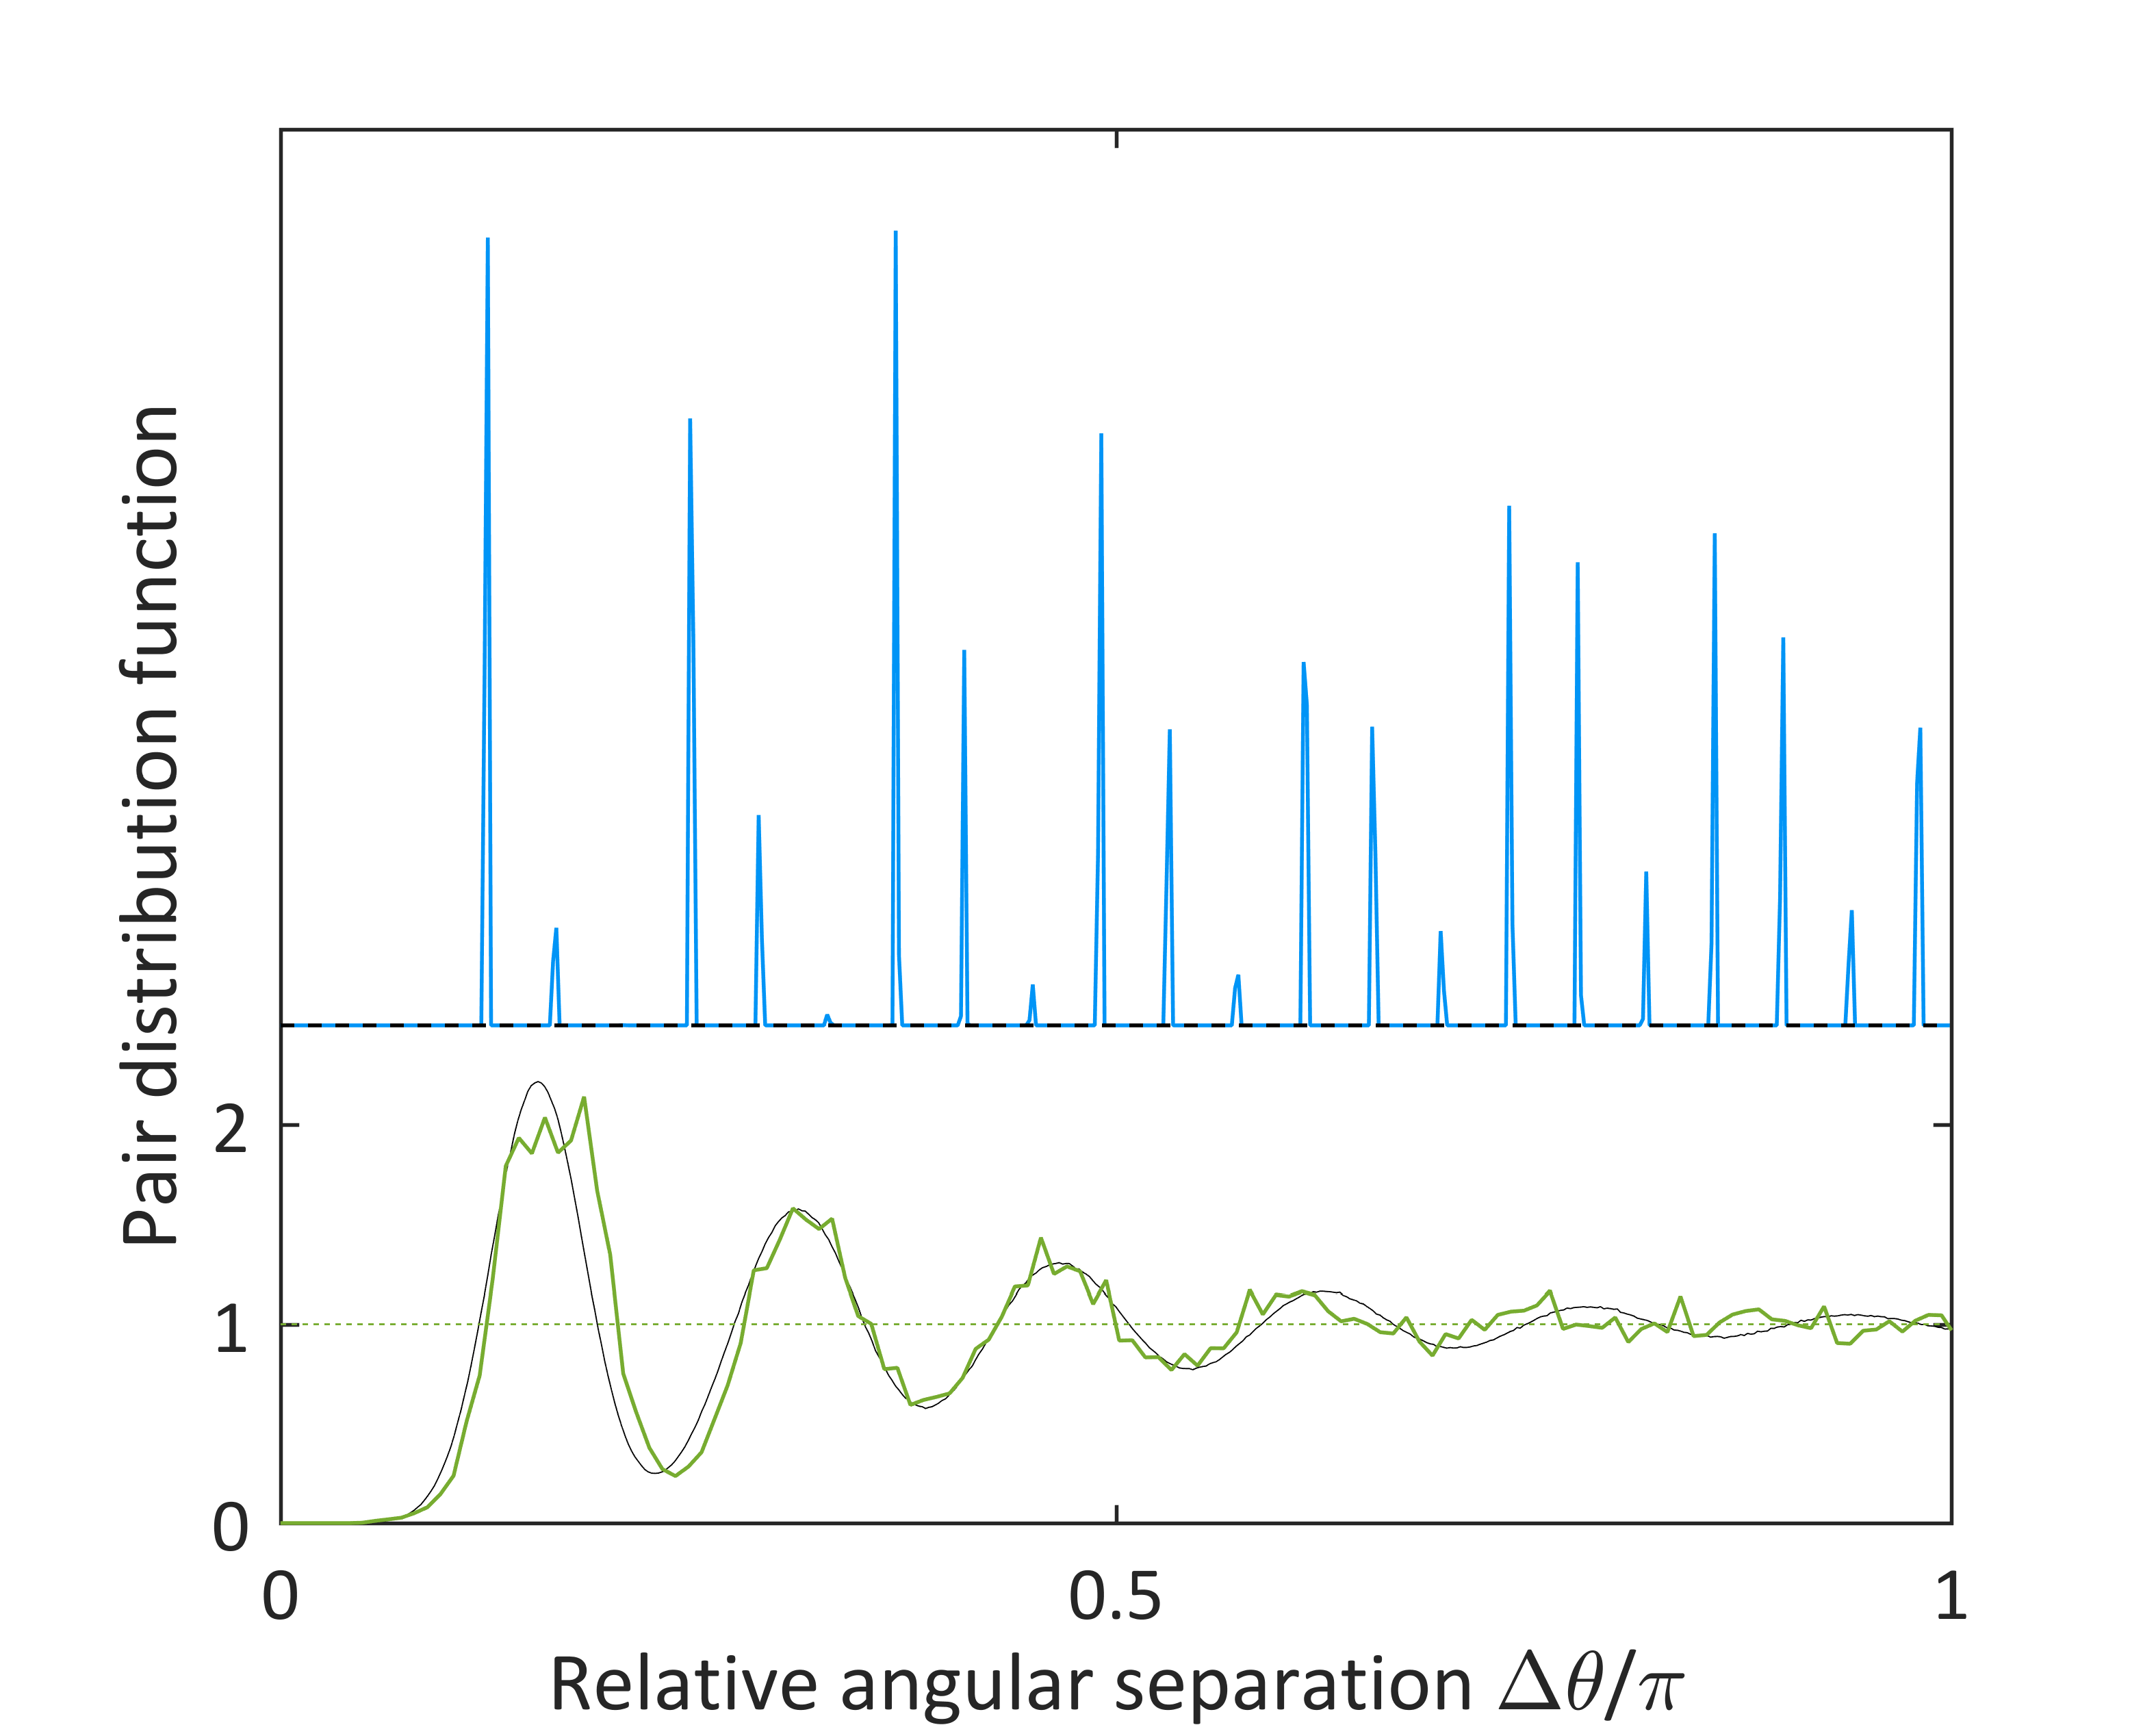
\includegraphics{\FigPath/Figures/SolitonCrystals/SCpdf.png}
	\end{center}
	\caption[Pair distribution function for soliton crystal generation]{\textbf{Pair distribution function for soliton crystal generation.} Average pair distribution functions calculated over 10,000 simulated scans across the resonance with (blue) and without (green) a mode crossing on mode 49. The width of the peaks in the discrete PDF is a single $\Delta\theta$ bin. The expected PDF of a simple one-dimensional soliton liquid (see main text) is plotted for comparison in black.}
	\label{fig:SCpdf}
\end{figure} 


 
\section{Soliton crystal configuration space}\label{sec:SCtaxonomy}

We observe a rich variety of soliton crystals explained by ordering in accordance with an extended background wave as described above. Operationally, we adjust the pump laser power to provide repeatable conditions for creating particular crystals; crystals exhibiting a greater number and variety of defects occur with increased laser power, which intensifies the fluctuations in the chaos that precedes crystal generation and provides less well-ordered initial conditions. Once a crystal is generated, it is stable to small adjustments in the pump power and detuning in accordance with the range of soliton existence shown in Fig. \ref{fig:MRLLEspace}, as the crystal structure is determined by the initial conditions for soliton formation rather than by an explicit dependence on pump power or detuning. 

Our interpretation of experimental data is based first on the fact that the LLE restricts the behavior of the field $\psi$ to either an extended pattern (primary comb pulse train or chaos) or an ensemble of solitons. When the measured experimental spectrum of a Kerr comb does not obviously correspond to a small number of solitons, then simultaneous experimental measurement of 1. A quiet repetition-rate tone when the spectrum of the photodetected power is analyzed, and 2. Single-FSR spacing in the spectrum indicate that the comb is a soliton crystal\footnote{These requirements are probably sufficient, but not necessary---for example, a defect-free crystal will exhibit multi-FSR spacing. Experimentally, the difference between such a crystal and a primary-comb pulse train lies in the parameters $\alpha$ and $F^2$ that place the pump laser \textit{either} in the regime for solitons or the regime for primary comb. However, these parameters are not necessarily straightforward to determine.}. To determine the temporal structure of a soliton crystal, we begin with the assumption that the spectrum corresponds to a soliton ensemble. Using the properties of the Fourier transform (e.g. linear superposition and the fact that a shift in time corresponds to a linear spectral phase shift), it is usually possible to deduce the configuration of pulses that must lead to the observed spectrum. Once the pulse train corresponding to the general structure of the spectrum has been deduced, the experimental spectrum can be compared to the spectrum of this pulse train calculated as an ensemble of solitons according to Eq. \ref{eq:LLEsolens}. This comparison reveals localized excess power in the experimental spectrum, which is evidence of a mode crossing. The strength of the mode crossing, controlled in the experiment by e.g. the taper-induced coupling between modes, is determined phenomenologically from the magnitude of the excess power and reduced comb-resonator detuning on a single mode is incorporated into a perturbed LLE as described in Sec. \ref{sec:crystallizationmechanism}. It is then verified that the pulse train whose spectrum matches the experimental data is a steady-state solution to this perturbed LLE, which requires the inter-soliton separations to be multiples of the period of the beat between the excess power and the pump laser. This period is $2\pi /\mu_\times$, where $\mu_\times$ is the mode number of the affected mode. Because this process connects the presence of excess power on a single optical mode of the Kerr-comb spectrum to the general shape of the spectrum, two observations that are not \textit{a priori} related, it provides strong evidence that the time-domain waveform of the crystal has been determined correctly.

The crystals we observe exhibit vacancies (Schottky defects), dislocations (Frenkel defects), disorder, or superstructure, or some combination thereof \cite{Ashcroft1976}. In a disordered crystal, the solitons still occupy lattice sites whose positions are determined by an avoided mode crossing in the resonator spectrum, but their distribution over these lattice sites varies without any apparent regular order or favored period. In this case, it is less straightforward to determine the pulse configuration from the shape of the spectrum. Instead, to determine the pulse configuration for a disordered crystal, we first identify excess power due to a mode crossing through observation of an asymmetry in the spectrum about the pump. The location of the excess power then fixes the allowed inter-soliton separations in the resonator, after which an exhaustive search is performed until a pulse train is found that yields the experimental spectrum. 

\begin{sidewaysfigure}[htpb]
	\begin{center}
		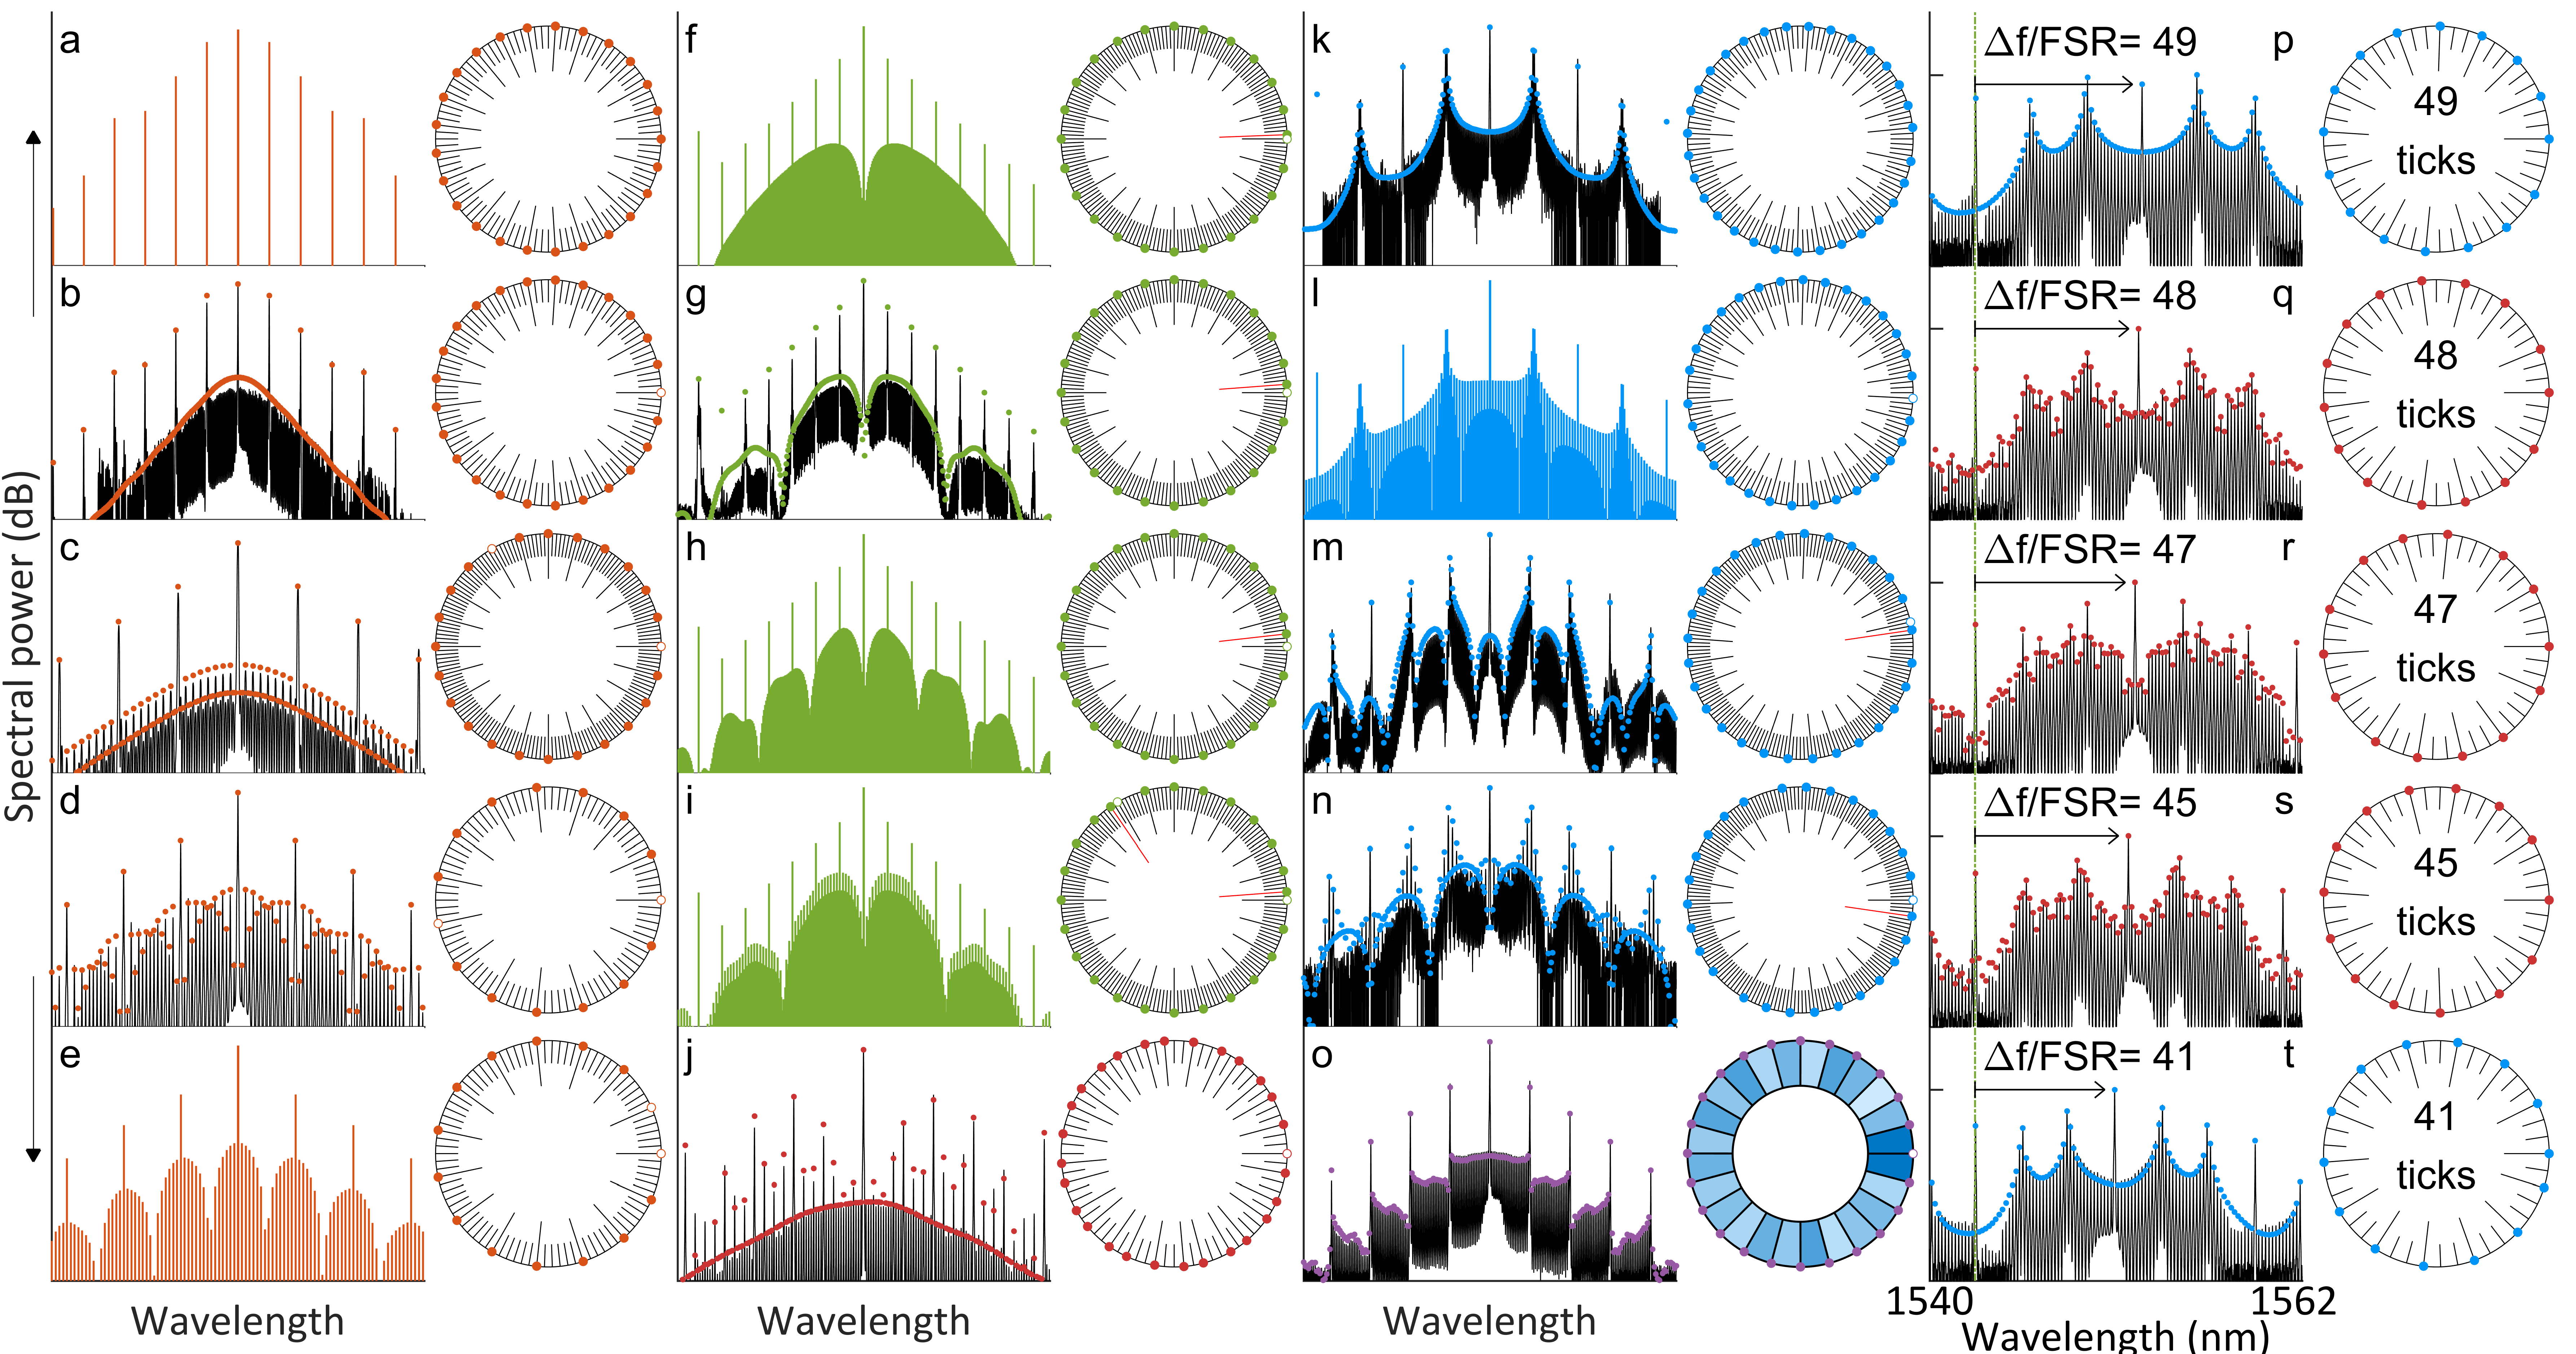
\includegraphics{\FigPath/Figures/SolitonCrystals/SCtaxonomy.png}
	\end{center}
	\caption[Taxonomy of soliton crystals]{\textbf{Taxonomy of soliton crystals.} Measured optical spectra are shown in black, with simulations in color. Schematic depictions of the soliton distribution in the resonator co-moving frame are shown to the right of each spectrum. Major ticks in the schematic diagrams indicate the location or expected location of a soliton. Minor ticks indicate lattice sites, corresponding to peaks of the extended background wave due to a mode crossing. (a) A perfect soliton crystal, consisting of 25 uniformly-distributed solitons. (b-e) Soliton crystals exhibiting vacancies. (f-i) Soliton crystals exhibiting Frenkel defects. Shifted solitons still occupy a lattice site. (j) A disordered crystal. (k-n) Crystals exhibiting superstructure. (o) A crystal with irregular inter-soliton spacings. Darker shading indicates a smaller inter-soliton spacing. The range in inter-soliton spacings is 3 $\%$ of the mean. (p-t) A series of crystals generated as the pump laser is moved progressively closer to the stabilizing mode crossing.}
	\label{fig:SCtaxonomy}
\end{sidewaysfigure}


Optical spectra for various observed and hypothetical soliton crystals are plotted in Fig. \ref{fig:SCtaxonomy}. We have simulated 13 of the experimental spectra as steady-state solutions to a perturbed LLE (this excludes crystal o); for 10 of these, the stabilizing mode crossing is visible in the data but not necessarily shown in the figure. For the other three the position of the mode crossing is inferred from the distribution of solitons and other crystal states observed in the same resonator.


We highlight the crystal plotted in Fig. \ref{fig:SCtaxonomy}n. This crystal exhibits both superstructure, with a superlattice period of $2\pi/3$ radians, and a Frenkel defect. Three identical supercells per resonator round-trip yield a spectrum that has light in optical modes spaced by three resonator FSR, because the waveform's period has been reduced threefold. The Frenkel defect, occurring once per round-trip, transfers a pulse from one supercell to another and contributes the single-FSR lobes to the spectrum. The result is three bursts of pulses containing 8, 9, and 10 solitons respectively. 	

Fig. \ref{fig:SCtaxonomy}o shows a soliton crystal with inter-soliton separations that are slightly irregular and that we have not simulated as a steady-state solution of any perturbed LLE. We expect that the formation of the crystal and the distribution of solitons are dictated by mode interactions, but that in this case our simple approximation of a perturbation to the LLE by a reduced comb-resonator detuning on a single comb mode is not appropriate.

Finally, we highlight the series of crystals plotted in Figs. \ref{fig:SCtaxonomy}p-\ref{fig:SCtaxonomy}t. This series of crystals was generated by moving the pump laser closer to a mode-crossing in steps of integer multiples of the resonator FSR. This data demonstrates the influence of the background beating between the pump laser and the mode crossing in determining the configuration of solitons in the resonator.





\section{Time-domain measurements of soliton crystals}
It is recognized in ultrafast optics that it is not generally possible to infer the time-domain waveform of an optical signal from its optical power spectrum without additional information \cite{Weiner2009}, because the spectrum contains no phase information. The LLE imposes restrictions on the possible time-domain field behaviors that can be exhibited, which can allow educated guesses to be made about the time-domain field based on the recorded optical spectrum, and we have been successful in modeling the observed spectra presented above as soliton ensembles. However, it is useful to confirm the LLE-assisted interpretation of experimental data both to strengthen the case for the LLE as a useful model for the system and to stay alert to the possibility of extra-LLE phenomena. 

To verify our time-domain interpretation of the spectra we record in experiment, we characterize the temporal intensity of soliton crystals using an optical cross-correlation measurement. A depiction of the approach and the results for measurement of the time-domain intensity of the crystal shown in Fig. \ref{fig:SCtaxonomy}j is shown in Fig. \ref{fig:SCxcorr}. We send the Kerr-comb output and an optical reference pulse train through a LiIO\textsubscript{3} crystal with a relative angle of 90\textsuperscript{o} between the beams. When the beams overlap in the crystal an amount of light proportional to the product of their intensities, at the sum of their frequencies, is emitted in a third direction. By measuring the average power of this emitted light while scanning the relative delay between the two beams, we measure the intensity cross-correlation between the crystal and the reference pulse.

In the limit of a $\delta$-function reference pulse, optical cross-correlation directly measures the time-domain waveform of an unknown signal. To approximate this limit, we perform cross-correlation measurements with a train of reference pulses that have duration comparable to that of the solitons, which allows us to precisely characterize soliton crystals. The reference pulse train is derived through electro-optic modulation (see Chapter \ref{chap:EOMCombs}) from the same laser that pumps the resonator, and the repetition rate of the reference pulse train is locked to the repetition rate of the Kerr-comb output. 

We generate crystals in a through-coupled configuration, which results in interference between the out-coupled solitons and the through-coupled pump that depends on the coupling condition and that effects the time-domain waveform that propagates away from the resonator. In this particular experiment the out-coupled solitons destructively interfere with the through-coupled pump, with the result that the solitons manifest as dips in the through-coupled intensity. To correct this, before cross-correlation we use a spatial light modulator to rotate the phase of the pump laser by $\pi$ so that it constructively interferes with the solitons, yielding solitons riding on top of a CW background. 



\begin{figure}[htpb]
	\begin{center}
		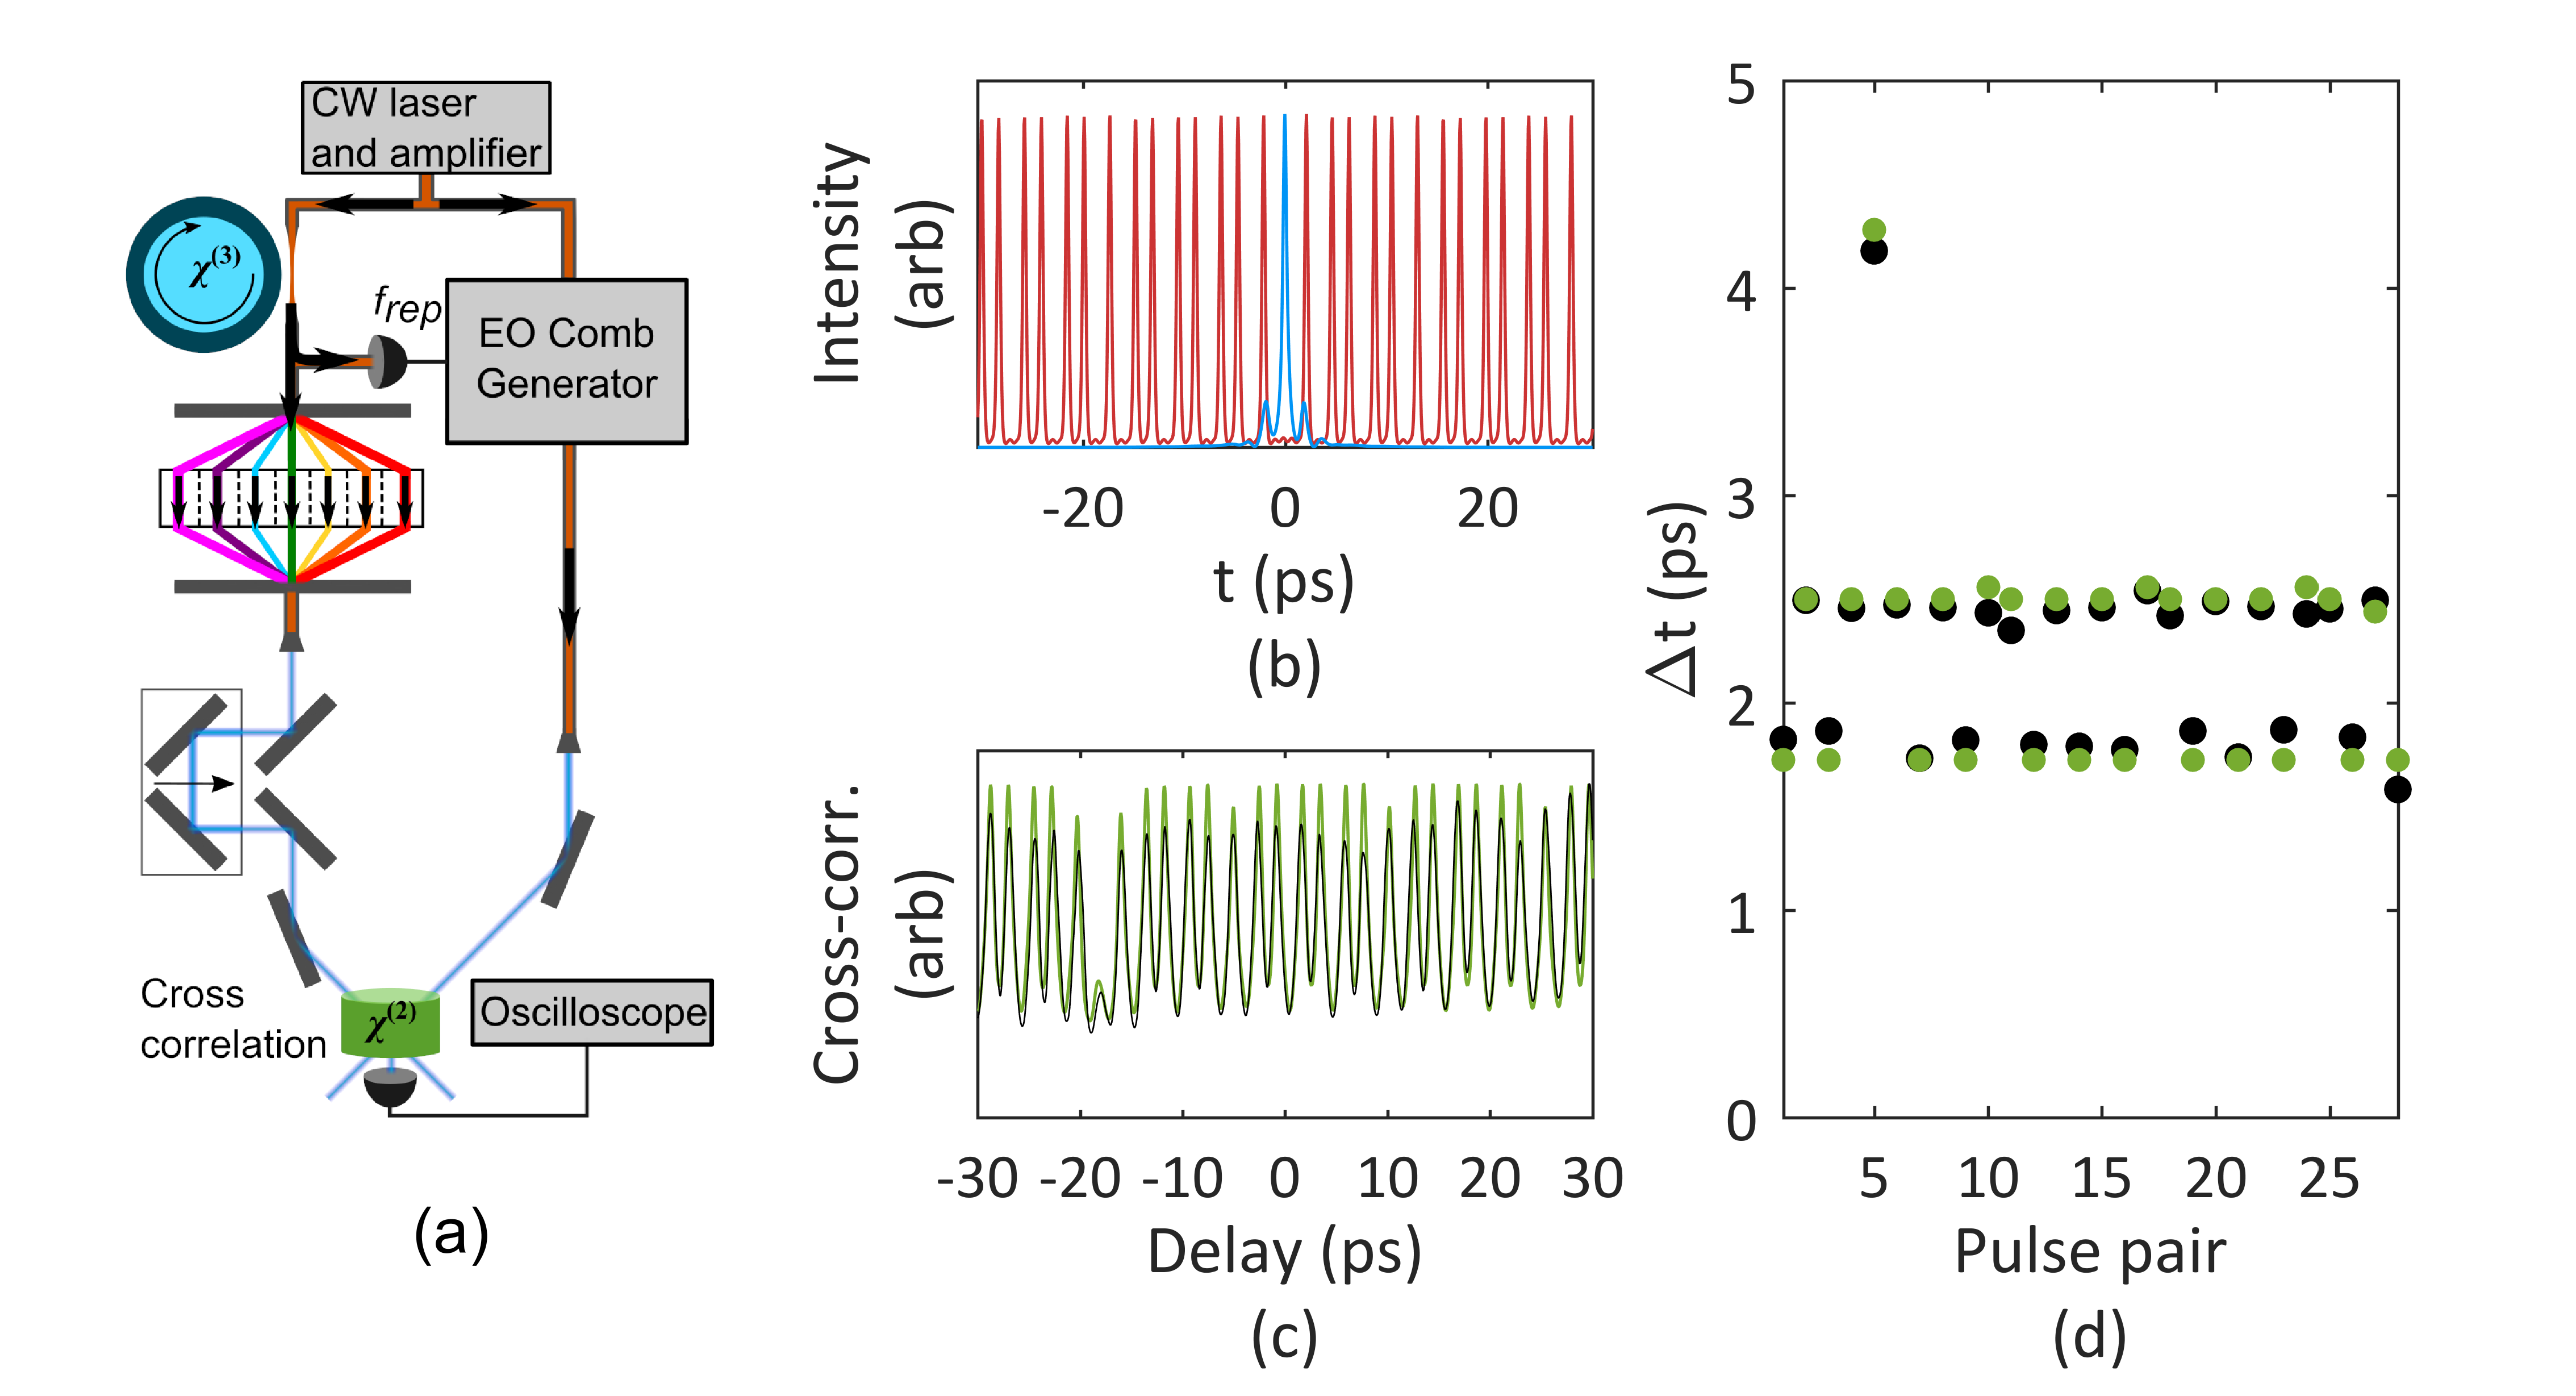
\includegraphics{\FigPath/Figures/SolitonCrystals/SCxcorr.png}
	\end{center}
	\caption[Cross-correlation characterization of a soliton crystal]{\textbf{Cross-correlation characterization of a soliton crystal.} Schematic depiction of the setup for using an electro-optic (EO) modulator comb as a reference pulse to measure the time-domain waveform of a soliton crystal. The $\chi^{(3)}$ (Kerr) and $\chi^{(2)}$ nonlinearities are indicated on the resonator and nonlinear crystal (LiIO\textsubscript{3}). A spatial light modulator is used to rotate the phase of the pump laser by $\pi$ after crystal generation to compensate for interference between the out-coupled soliton crystal and the through-coupled pump light. The soliton crystal and the EO modulator comb share a pump laser, and the repetition frequency $f_{rep}$ of the EOM comb is locked to that of the crystal. Varying the relative delay in one arm of this interferometer enables measurement of the intensity cross-correlation between the soliton crystal and the reference pulse. (b)  Simulated crystal (red) and reference (blue) intensity profiles. (c) Measured (black) and simulated (green) cross-correlation signals. The contrast between peaks of the cross-correlation signal, for both theory and experiment, is limited by the duration and shape of the reference pulse and increases between soliton pairs with larger temporal separations. (d) Temporal separations between adjacent peaks for the measured (black) and simulated (green) cross-correlation signals. Mean fractional error is 3.5~$\%$.}
	\label{fig:SCxcorr}
\end{figure} 

 
The cross-correlation of the disordered crystal shown in Fig. \ref{fig:SCtaxonomy}j with the reference pulse train confirms our interpretation of the spectral data for this crystal. Fig. \ref{fig:SCxcorr}b shows the simulated time-domain waveforms of the reference pulse and the crystal, and Fig. \ref{fig:SCxcorr}c shows measured and simulated cross-correlation signals. The temporal spacing between the peaks of the cross-correlation signals is shown in Fig. \ref{fig:SCxcorr}d, where a high degree of agreement between the data and the simulation is observed. 

The simulated cross-correlation signal is sensitive to the intensity profile of the reference pulse. We can measure only its intensity autocorrelation, which we combine with our knowledge of its production to estimate the intensity profile. To demonstrate that the validity of the results we present here is not sensitive to the exact assumptions we make about the intensity profile, we have also simulated the intensity cross-correlation resulting from an assumed Gaussian reference pulse with the same autocorrelation width as is measured for the reference pulse. The resulting simulated cross-correlation does not qualitatively agree as well with the experimental data in the depths of the wells between peaks because it does not contain satellite pulses which contribute to the variations in this depth, but the quantitative comparison of the temporal spacing between peaks is similar: the mean (maximum) normalized error between experiment and theory is 3.5 $\%$ (9.1 $\%$) for the assumed electro-optic comb pulse and 4.8 $\%$ (10.6 $\%$) for the Gaussian pulse.






